\section{Prototipo de Alta Fidelidad}
\noindent El prototipo de Leodega es una aplicación web de alta fidelidad \textbf{funcional} (no un mockup estático), desarrollada en React~19 con TypeScript y Tailwind CSS, y desplegada y navegable en \url{https://darwin4050e.github.io/PrototipoLeodega/}. El sistema soporta tres roles principales -- \textbf{Cliente}, \textbf{Gestor de Almacenamiento} (arrendador) y \textbf{Administrador} --, cada uno con su propio flujo de interacción. A continuación se documenta el flujo de ventanas (navegación) y las pantallas principales del prototipo, organizadas por rol.

\subsection{Flujo de Ventanas del Prototipo}
\begin{figure}[H]
    \centering
    \DiagramaImagen{0.98}{0.5}{imagenes/flujo_ventanas.png}
    \caption{Flujo de ventanas del prototipo de alta fidelidad}
    \label{fig:flujo_ventanas}
\end{figure}
\noindent\textbf{Descripción:} El usuario llega a la Landing Page y se registra o inicia sesión; tras seleccionar su perfil (Cliente, Gestor o Administrador), accede al flujo correspondiente a su rol: el Cliente navega el catálogo hasta completar una reserva en tres pasos (Detalle, Pago, Comprobante) y luego gestiona sus reservas, mensajes e inventario; el Gestor administra sus bodegas publicadas, las publica en un asistente de 7 pasos, y da seguimiento a reservas recibidas, mensajes y calendario; el Administrador supervisa el dashboard, aprueba o rechaza bodegas, y gestiona cuentas, reportes y mensajes.

\bigskip
{\sloppy\noindent\textbf{Herramienta utilizada:} \textit{React 19 + TypeScript + Tailwind CSS} (prototipo funcional real desplegado, no un mockup estático de una herramienta de diseño). Diagrama de flujo de ventanas elaborado con \textit{PlantUML v1.2026.6} (motor Graphviz/\texttt{dot}). Prototipo: \url{https://darwin4050e.github.io/PrototipoLeodega/}. Fuente del diagrama: \url{recursos/diagramas_uml/flujo_ventanas.puml}.\par}
\clearpage

\subsection{Capturas de Pantalla}

\subsubsection{Pantallas Generales}
\noindent Pantallas compartidas por todos los tipos de usuario: página de inicio pública, flujo de autenticación y selección de perfil.

\begin{figure}[H]
    \centering
    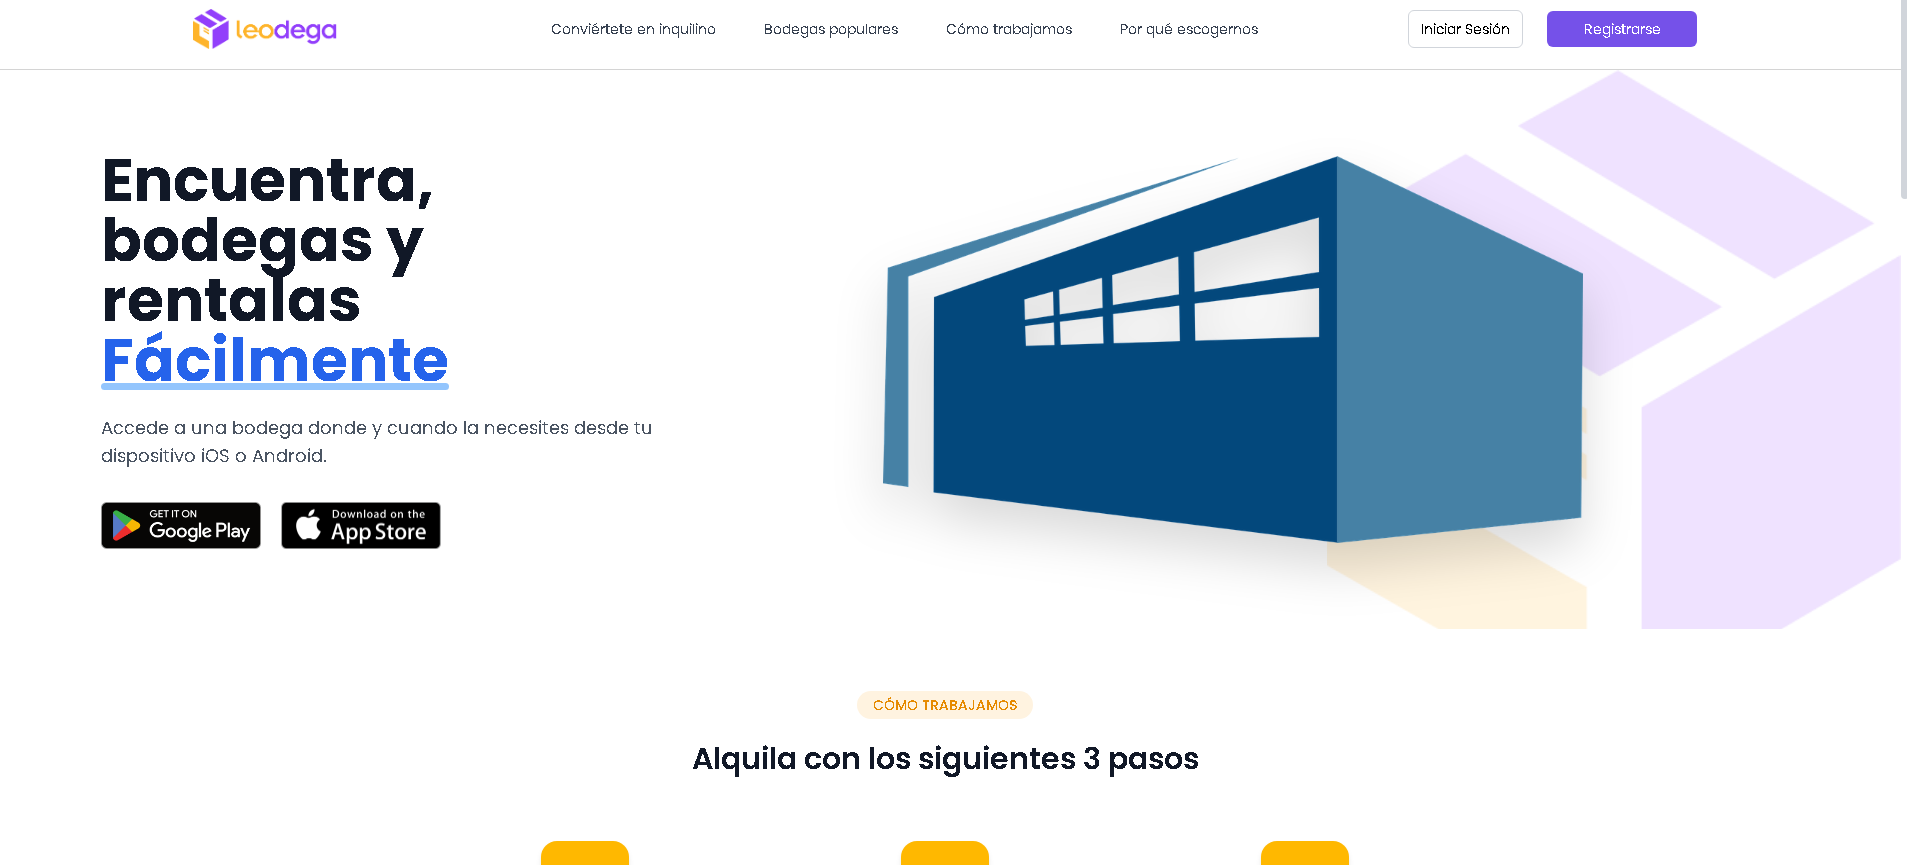
\includegraphics[width=\linewidth]{imagenes/fig01_landing_hero.png}
    \caption{Landing Page: sección hero con la propuesta de valor y accesos a las plataformas móviles.}
    \label{fig:landing_hero}
\end{figure}

\begin{figure}[H]
    \centering
    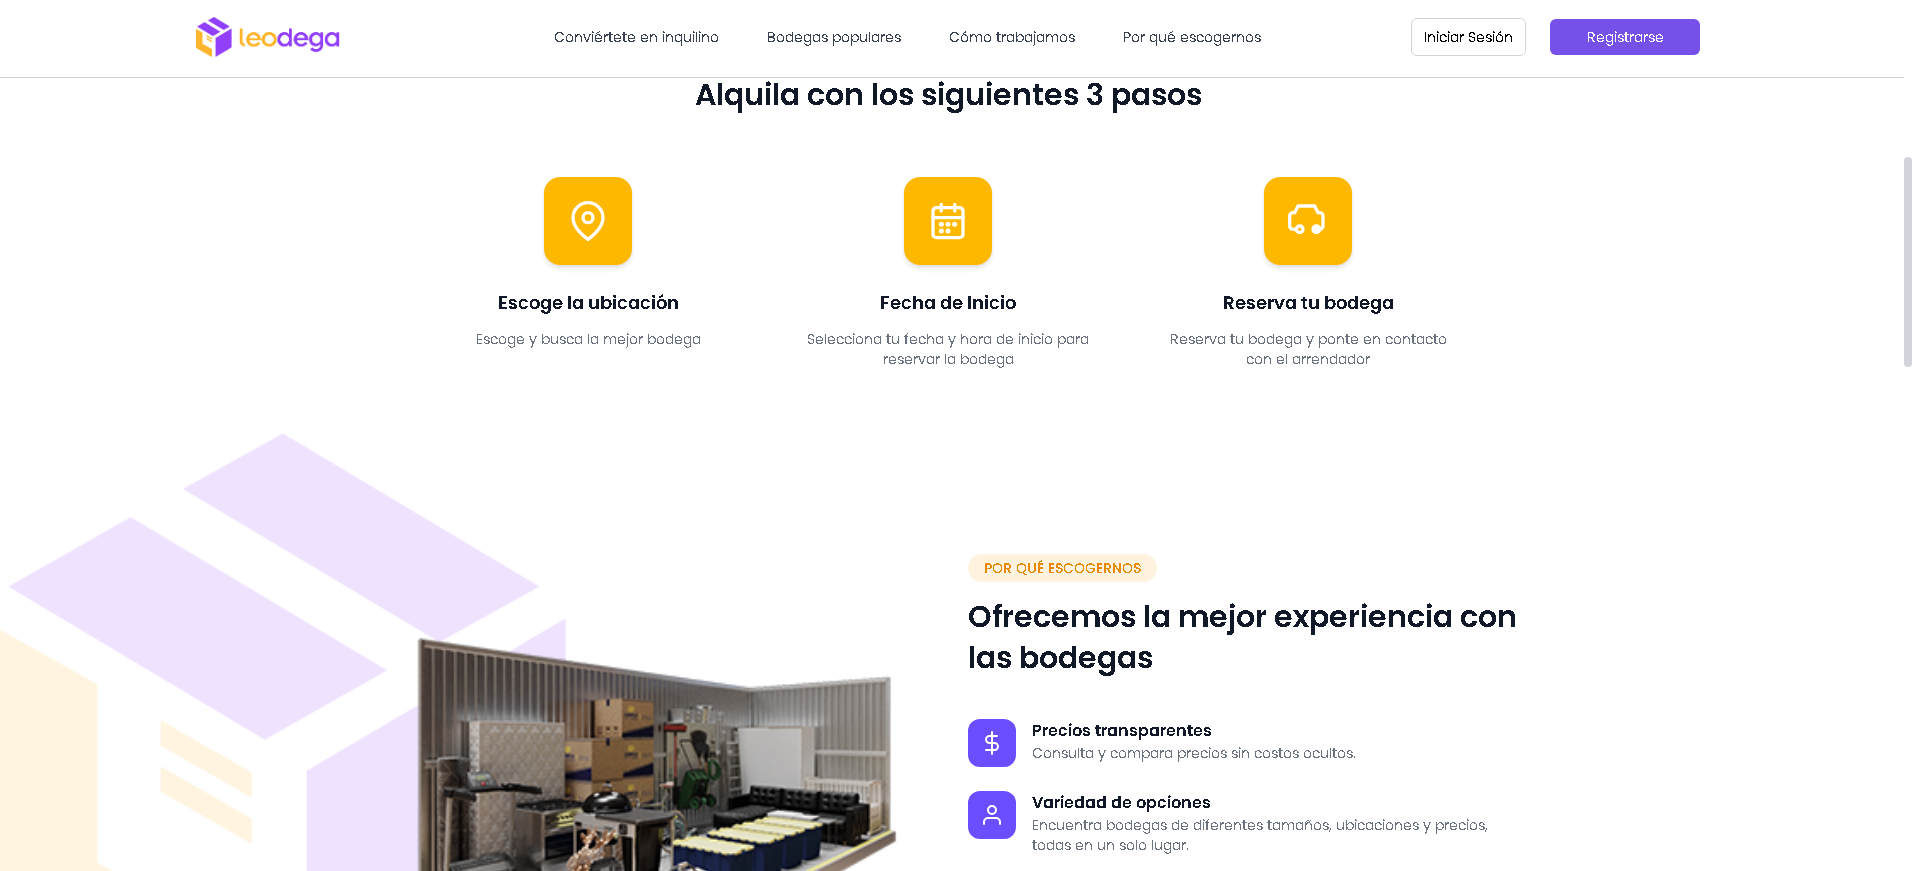
\includegraphics[width=\linewidth]{imagenes/fig02_how_it_works.png}
    \caption{Landing Page: sección ``Cómo Funciona'', el proceso de alquiler de bodegas en tres pasos.}
    \label{fig:how_it_works}
\end{figure}

\begin{figure}[H]
    \centering
    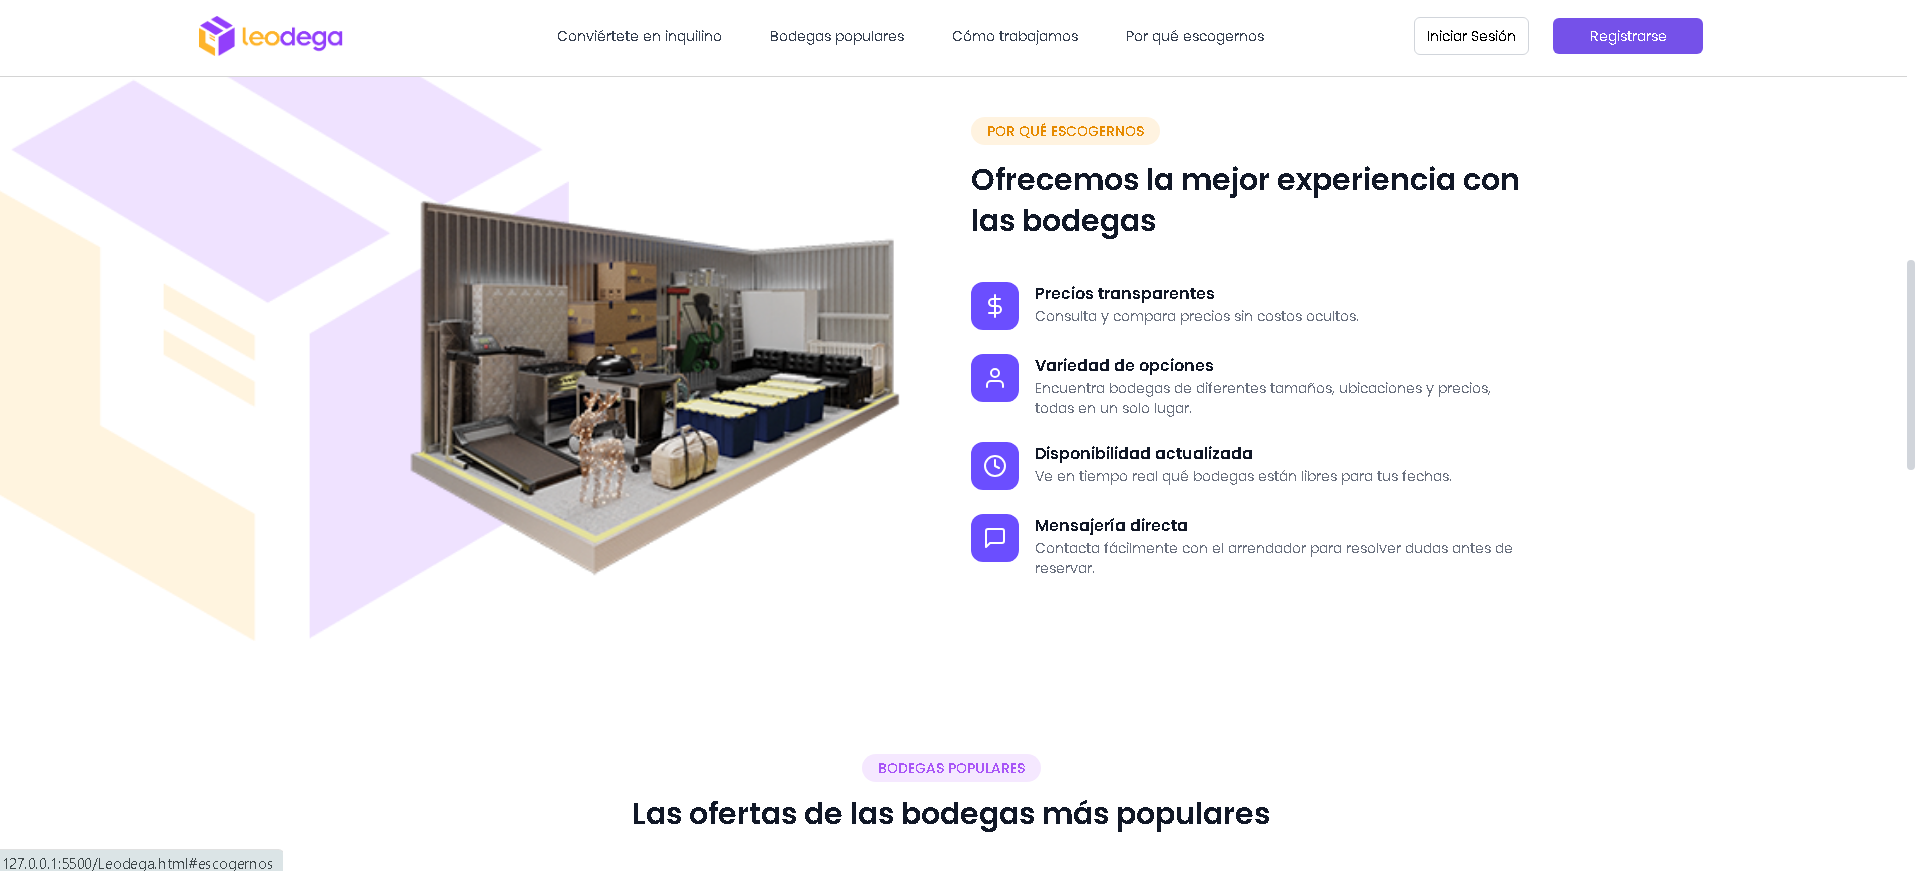
\includegraphics[width=\linewidth]{imagenes/fig03_why_choose_us.png}
    \caption{Landing Page: sección ``Por Qué Elegirnos'', con los diferenciadores clave de la plataforma.}
    \label{fig:why_choose_us}
\end{figure}

\begin{figure}[H]
    \centering
    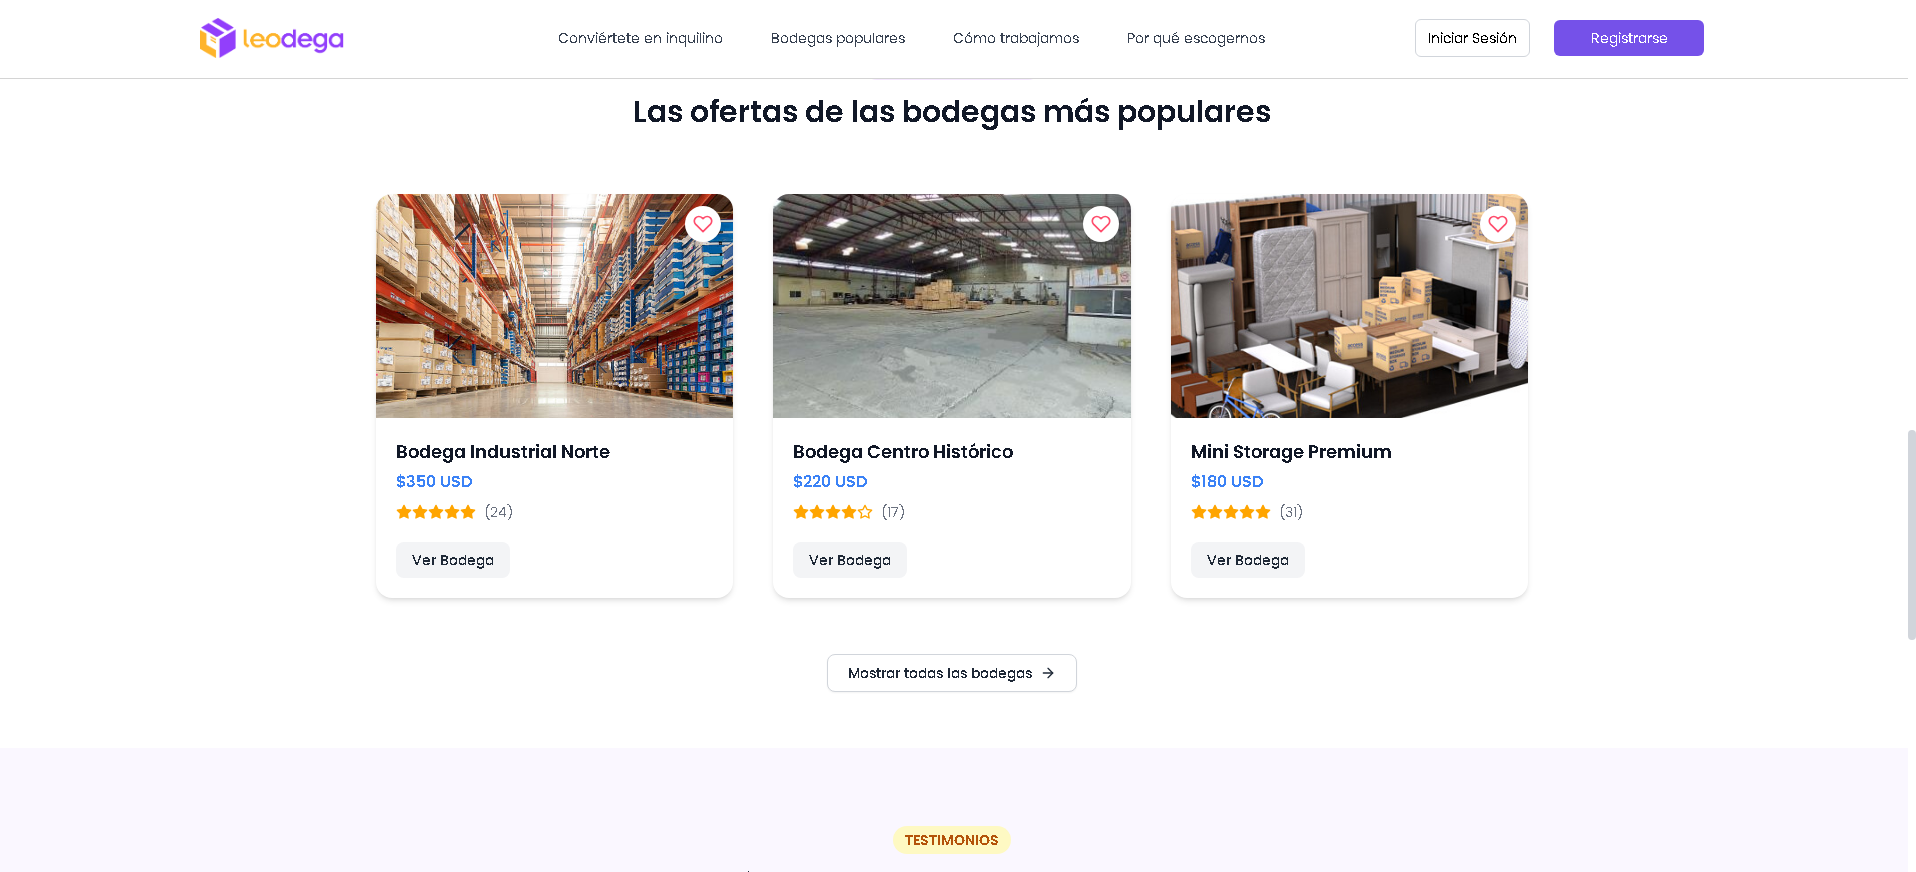
\includegraphics[width=\linewidth]{imagenes/fig04_popular_warehouses.png}
    \caption{Landing Page: sección ``Bodegas Populares'', publicaciones destacadas con precio y calificación.}
    \label{fig:popular_warehouses}
\end{figure}

\noindent\textbf{Autenticación.} El flujo de autenticación permite crear una cuenta nueva o iniciar sesión con credenciales propias o mediante proveedores externos (Facebook, Google, Apple).

\begin{figure}[H]
    \centering
    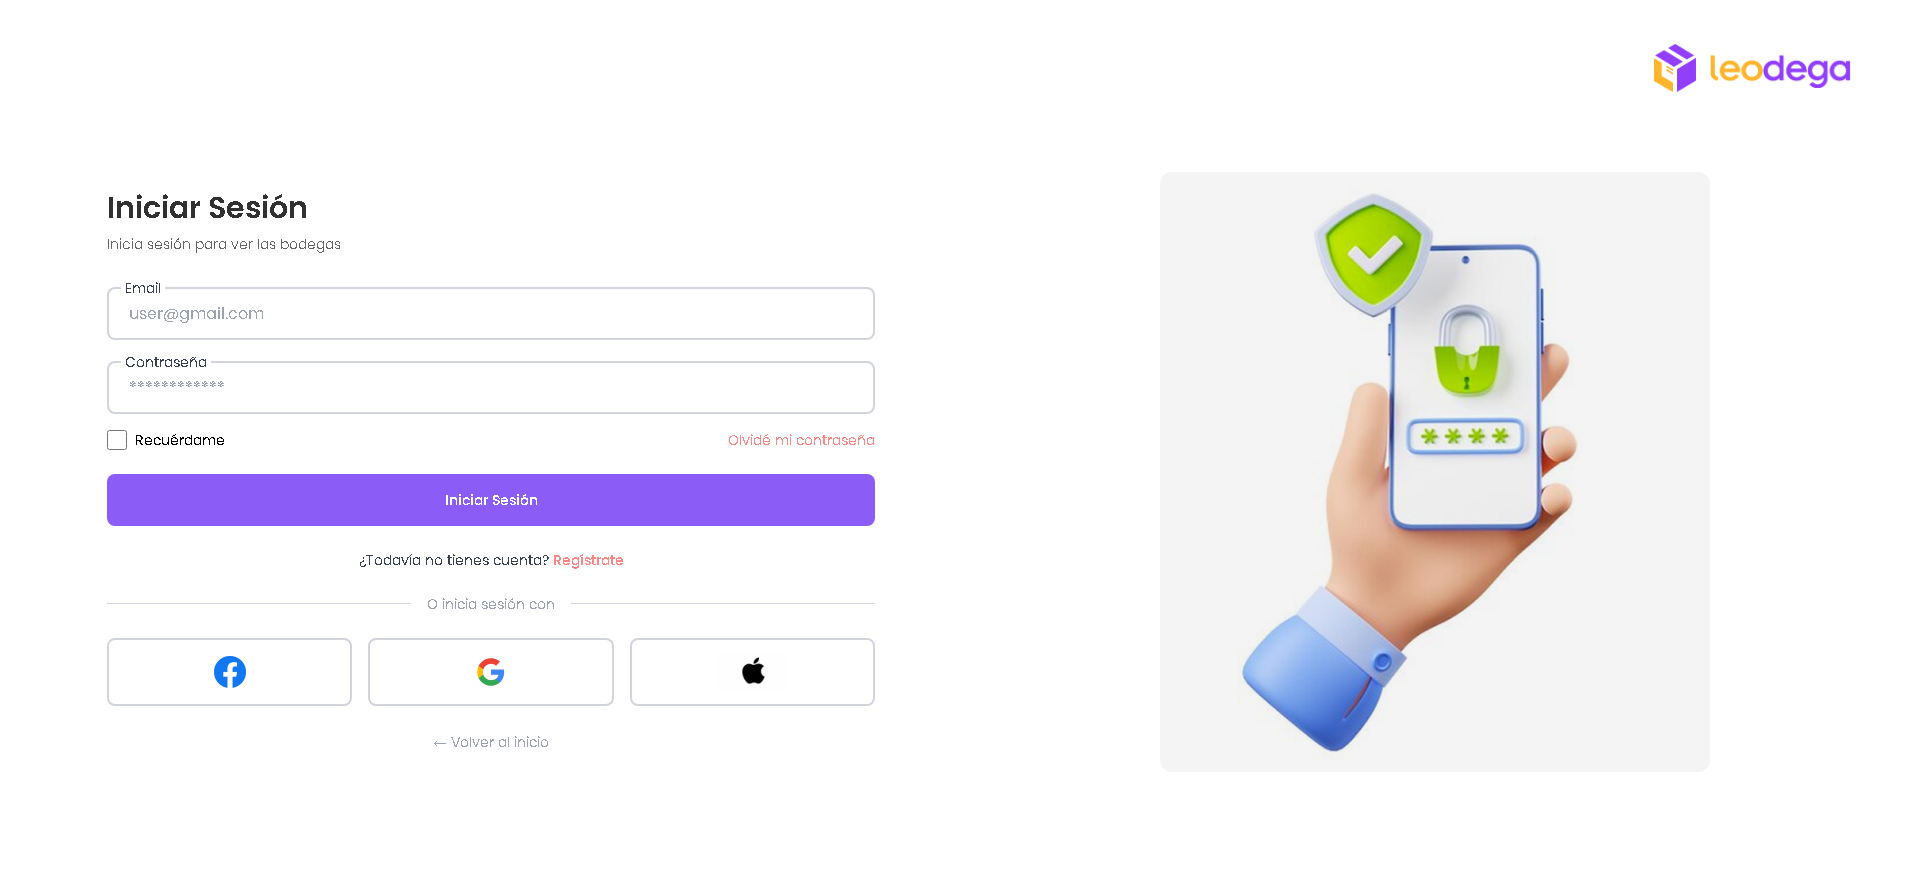
\includegraphics[width=0.85\linewidth]{imagenes/fig05_login.png}
    \caption{Pantalla de inicio de sesión con formulario de correo/contraseña y opciones de login social.}
    \label{fig:login}
\end{figure}

\begin{figure}[H]
    \centering
    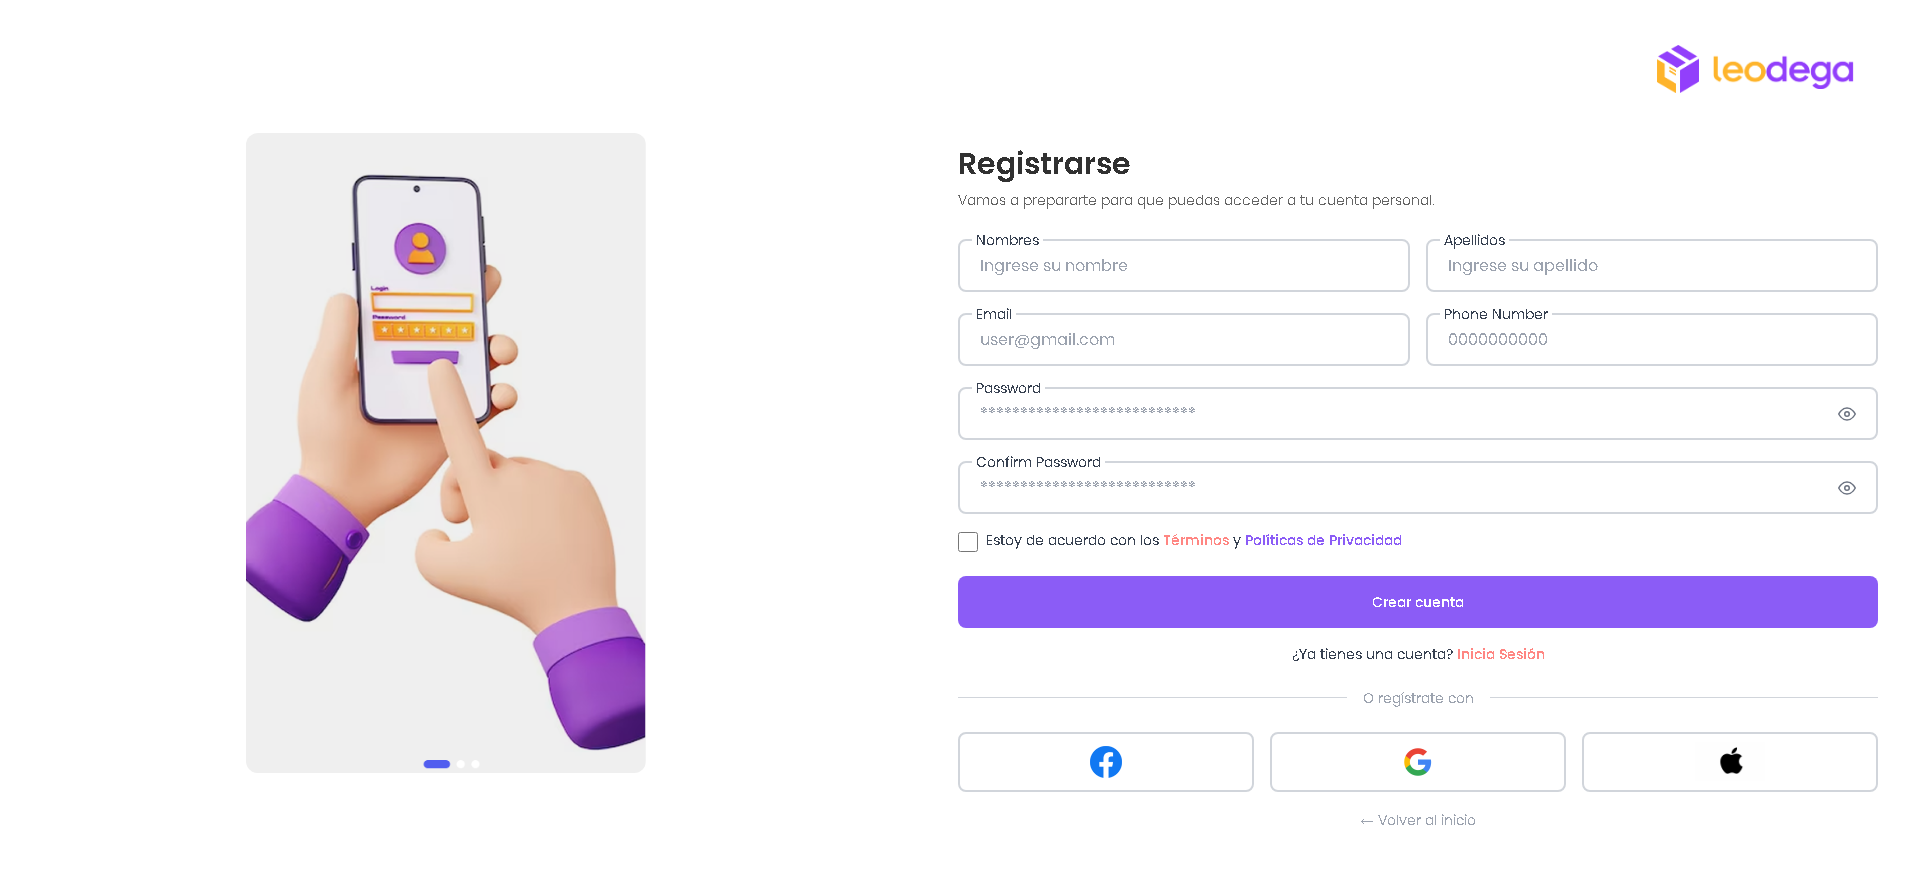
\includegraphics[width=0.85\linewidth]{imagenes/fig06_registration.png}
    \caption{Pantalla de registro: formulario de creación de cuenta con datos personales y confirmación de contraseña.}
    \label{fig:registration}
\end{figure}

\begin{figure}[H]
    \centering
    
\includegraphics[width=0.6\linewidth]{imagenes/fig07_profile_selection.png}
    \caption{Selección de perfil de usuario: Cliente, Gestor de Almacenamiento o Administrador.}
    \label{fig:profile_selection}
\end{figure}
\clearpage

\subsubsection{Cliente}
\noindent El flujo del Cliente le permite buscar y filtrar bodegas disponibles, ver su información detallada, completar el proceso de reserva y pago, y gestionar sus alquileres activos.

\begin{figure}[H]
    \centering
    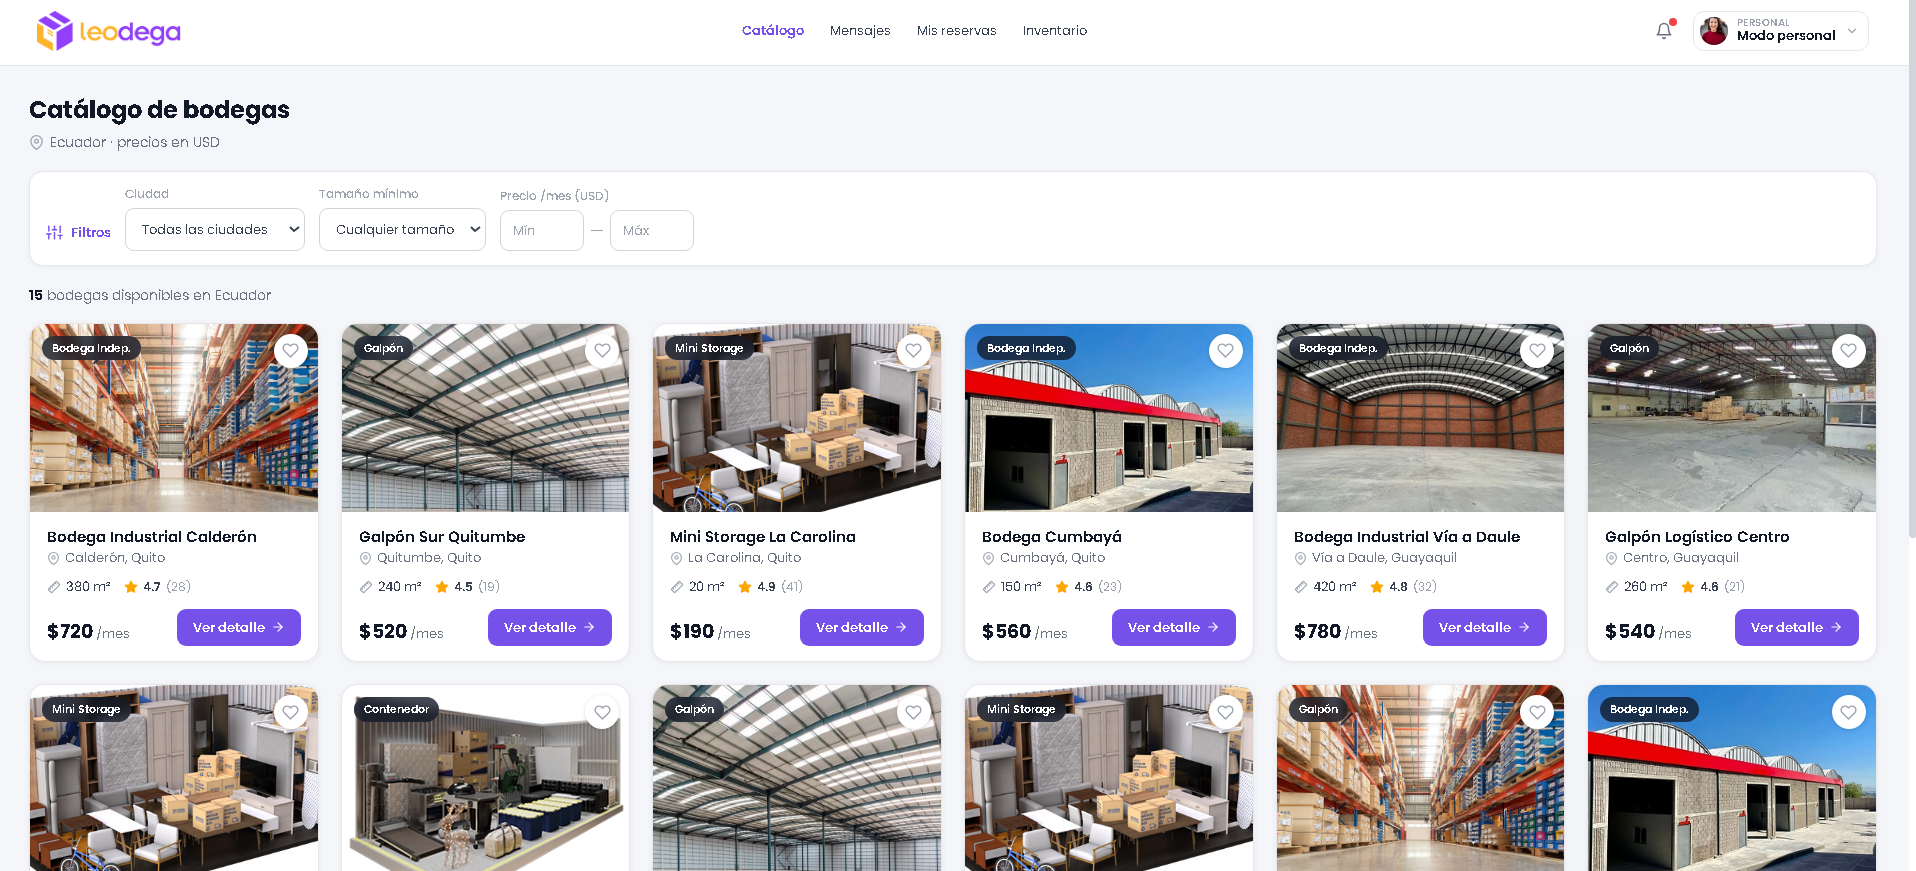
\includegraphics[width=\linewidth]{imagenes/fig08_catalog.png}
    \caption{Catálogo de Bodegas: vista de cuadrícula con filtros de ciudad, tamaño y precio (15 publicaciones).}
    \label{fig:catalog}
\end{figure}

\begin{figure}[H]
    \centering
    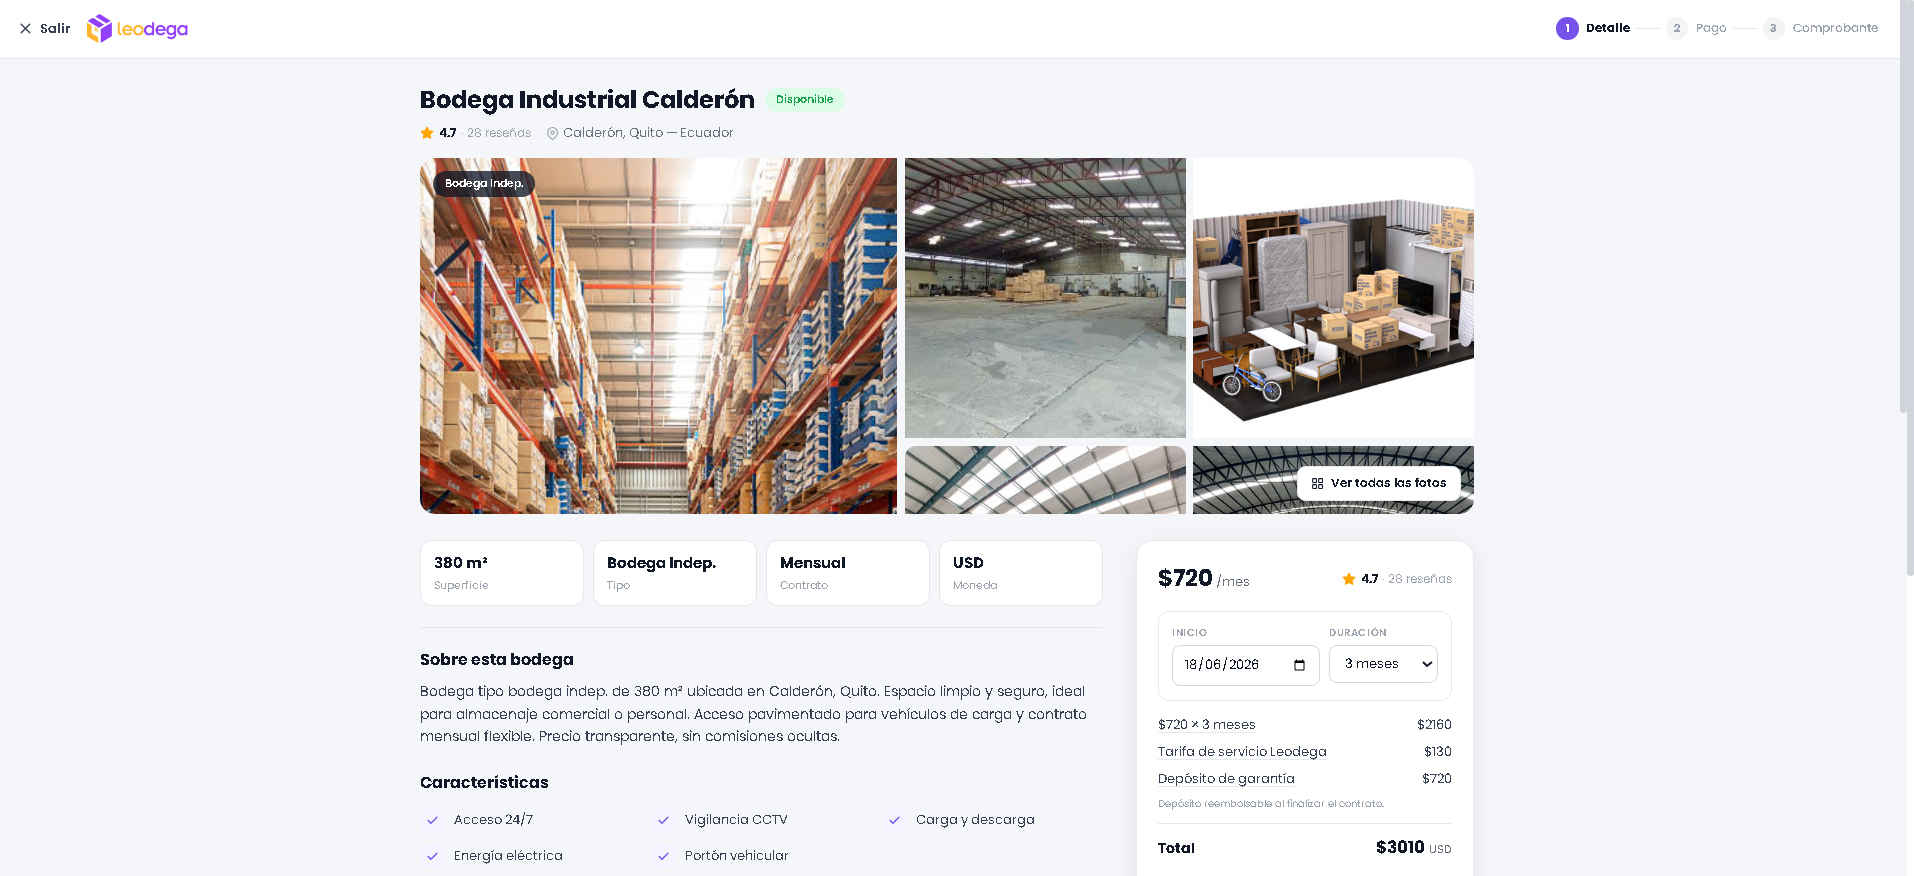
\includegraphics[width=\linewidth]{imagenes/fig09_warehouse_detail.png}
    \caption{Detalle de Bodega: galería de fotos, características y resumen de costos (Paso 1 del flujo de reserva).}
    \label{fig:warehouse_detail}
\end{figure}

\begin{figure}[H]
    \centering
    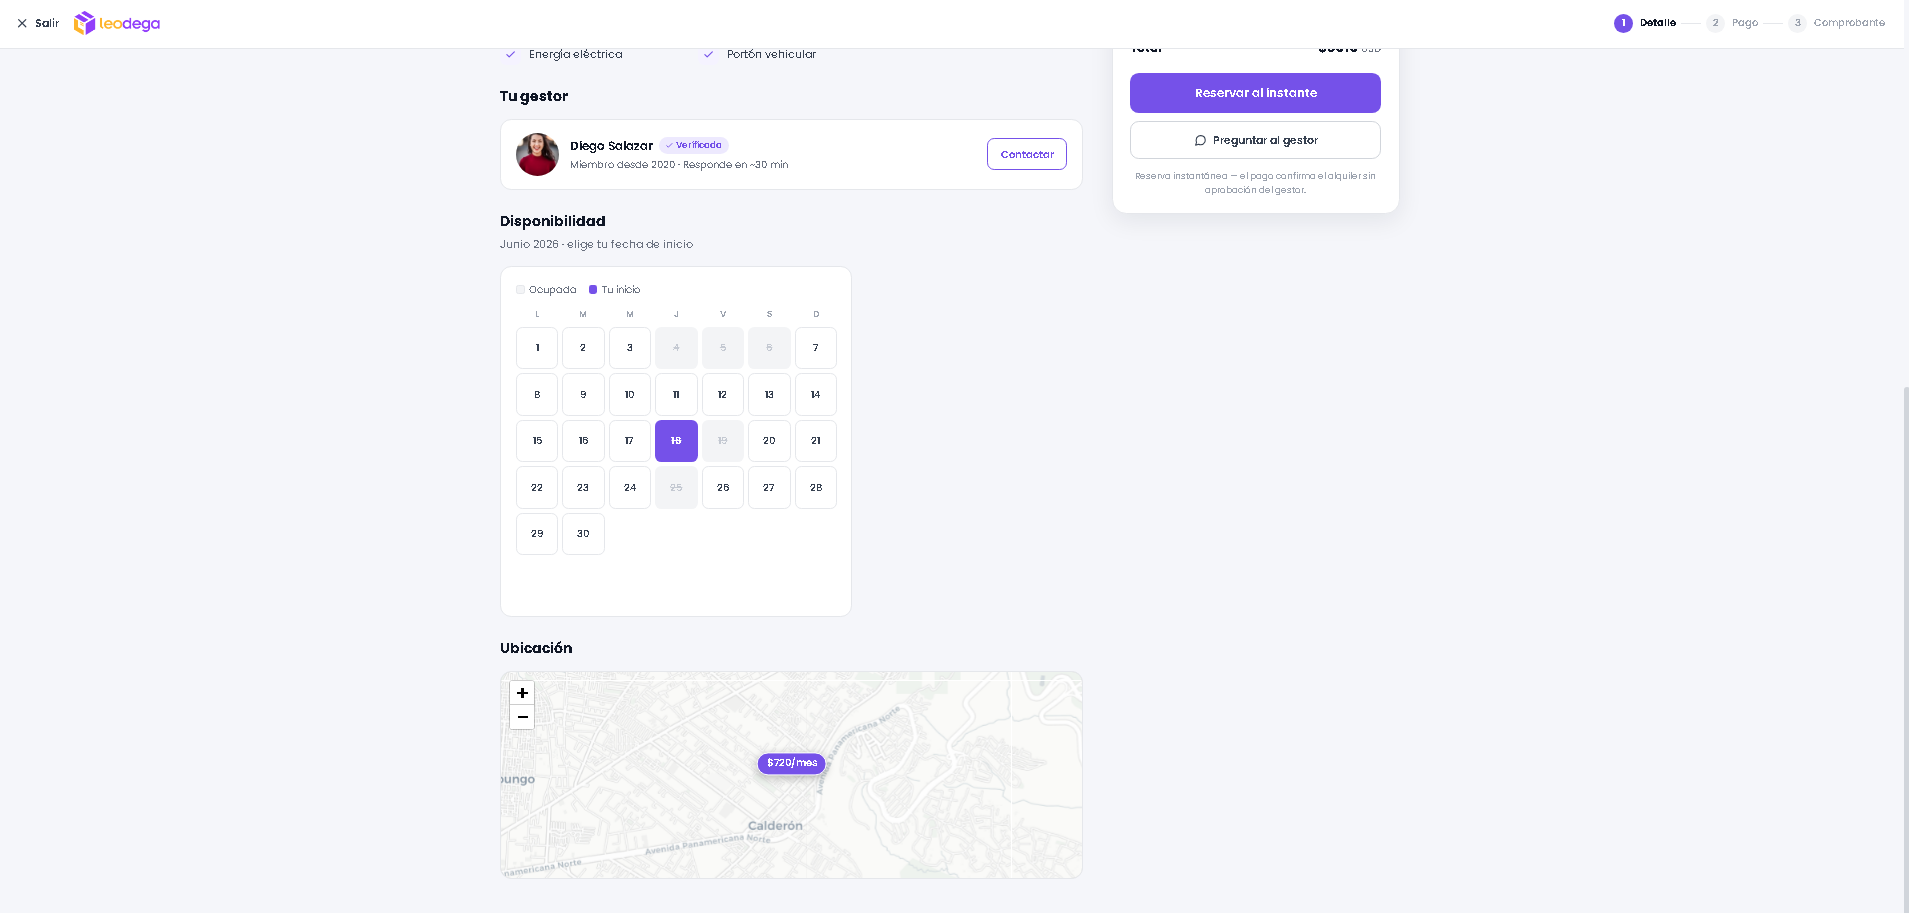
\includegraphics[width=\linewidth]{imagenes/fig10_warehouse_calendar.png}
    \caption{Detalle de Bodega: información del gestor, calendario de disponibilidad y mapa de ubicación.}
    \label{fig:warehouse_calendar}
\end{figure}

\begin{figure}[H]
    \centering
    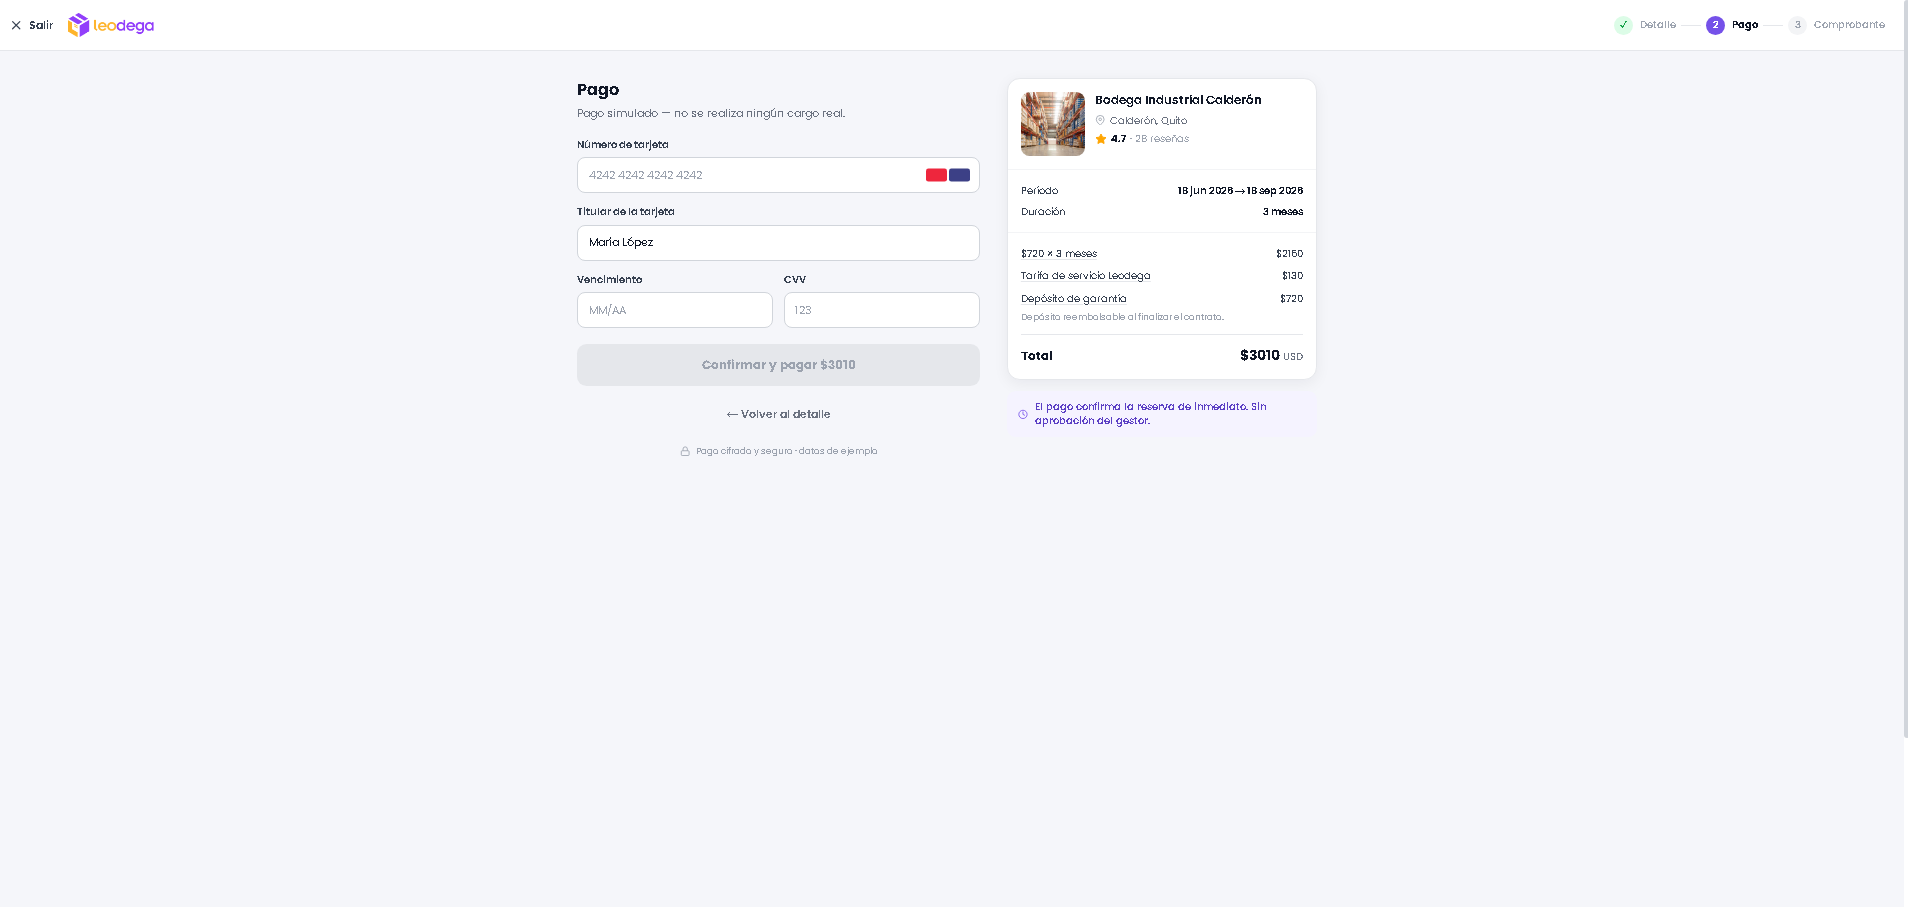
\includegraphics[width=\linewidth]{imagenes/fig11_payment.png}
    \caption{Paso 2 -- Pago: formulario de datos de tarjeta y resumen del costo total (\$3.010 USD).}
    \label{fig:payment}
\end{figure}

\begin{figure}[H]
    \centering
    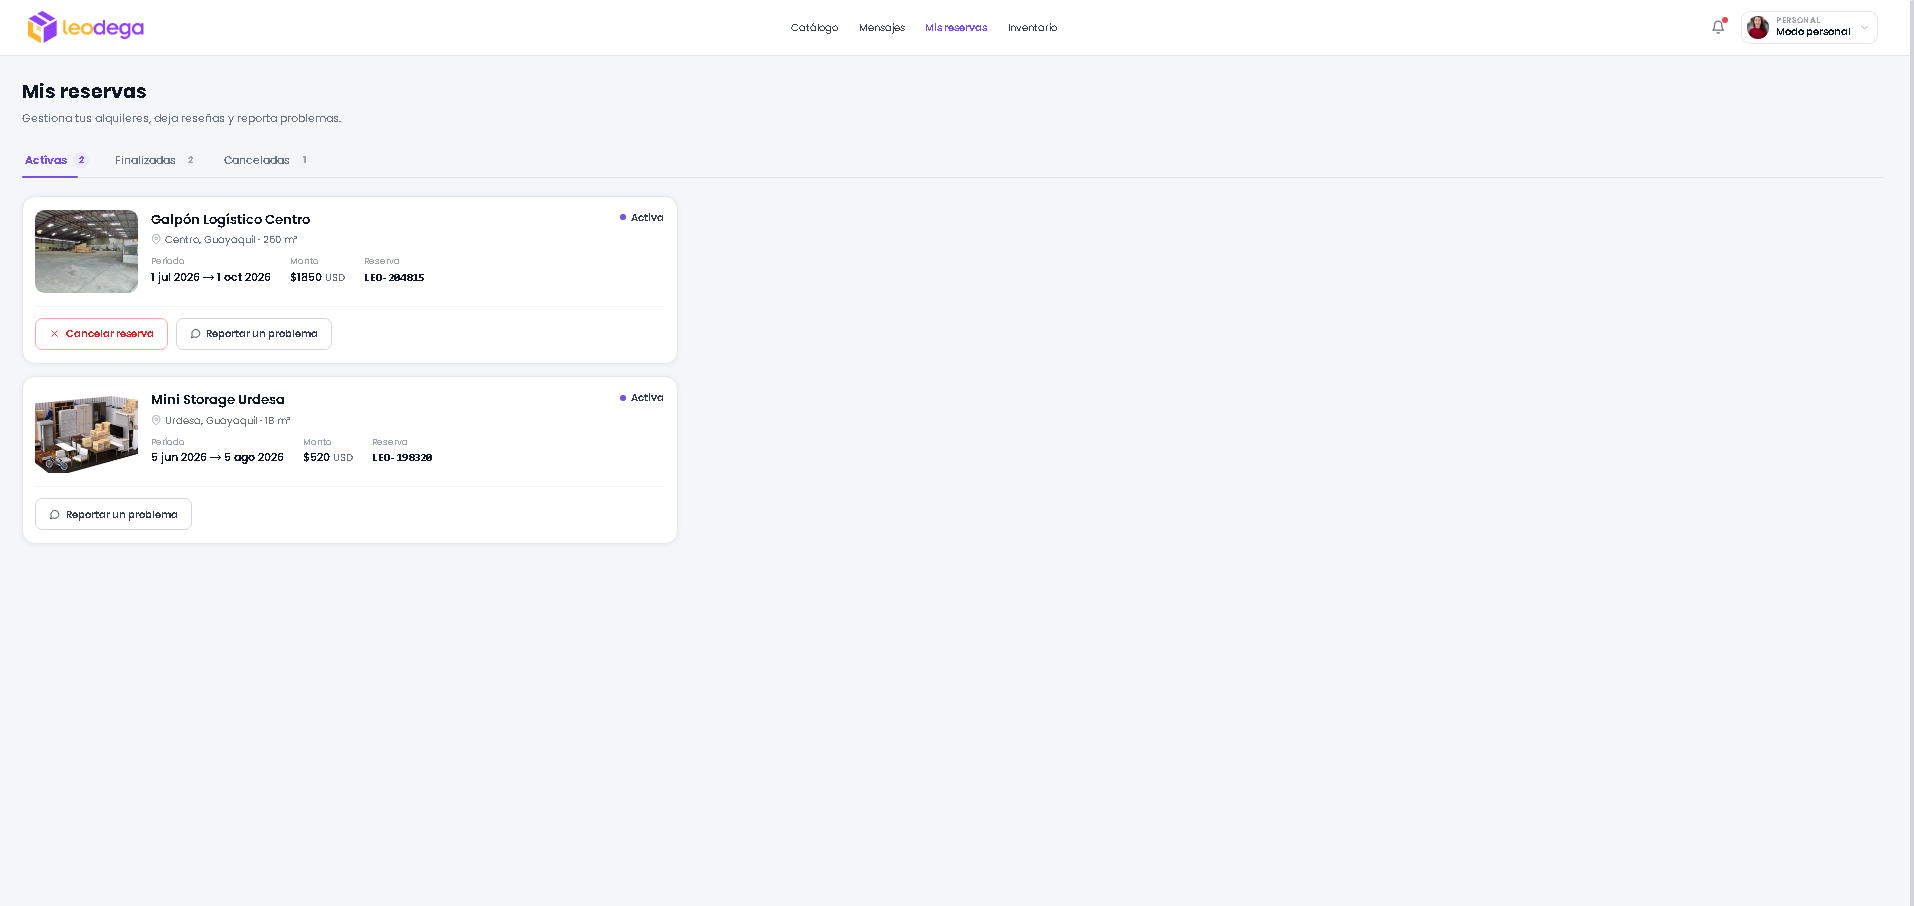
\includegraphics[width=\linewidth]{imagenes/fig12_my_bookings.png}
    \caption{Mis Reservas: lista de alquileres activos con período, monto y código de referencia de la reserva.}
    \label{fig:my_bookings}
\end{figure}

\begin{figure}[H]
    \centering
    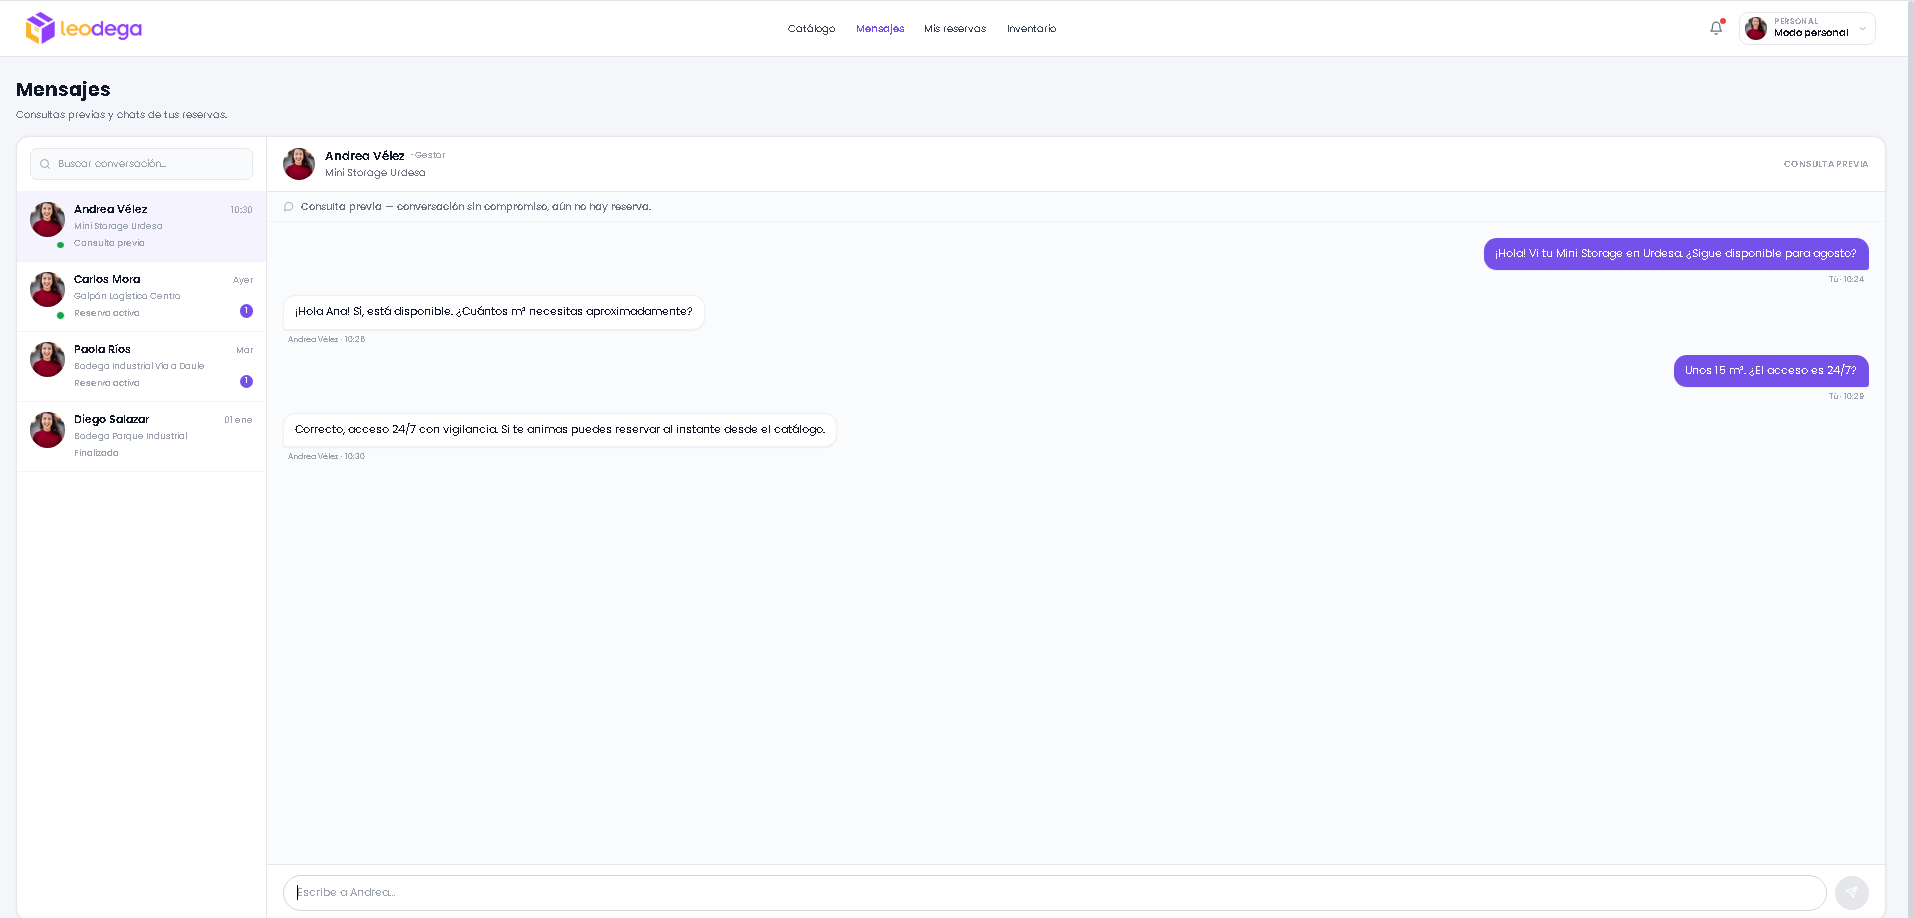
\includegraphics[width=\linewidth]{imagenes/fig13_tenant_messages.png}
    \caption{Mensajes del Cliente: bandeja de entrada con conversaciones por bodega y chat en tiempo real con el gestor.}
    \label{fig:tenant_messages}
\end{figure}

\begin{figure}[H]
    \centering
    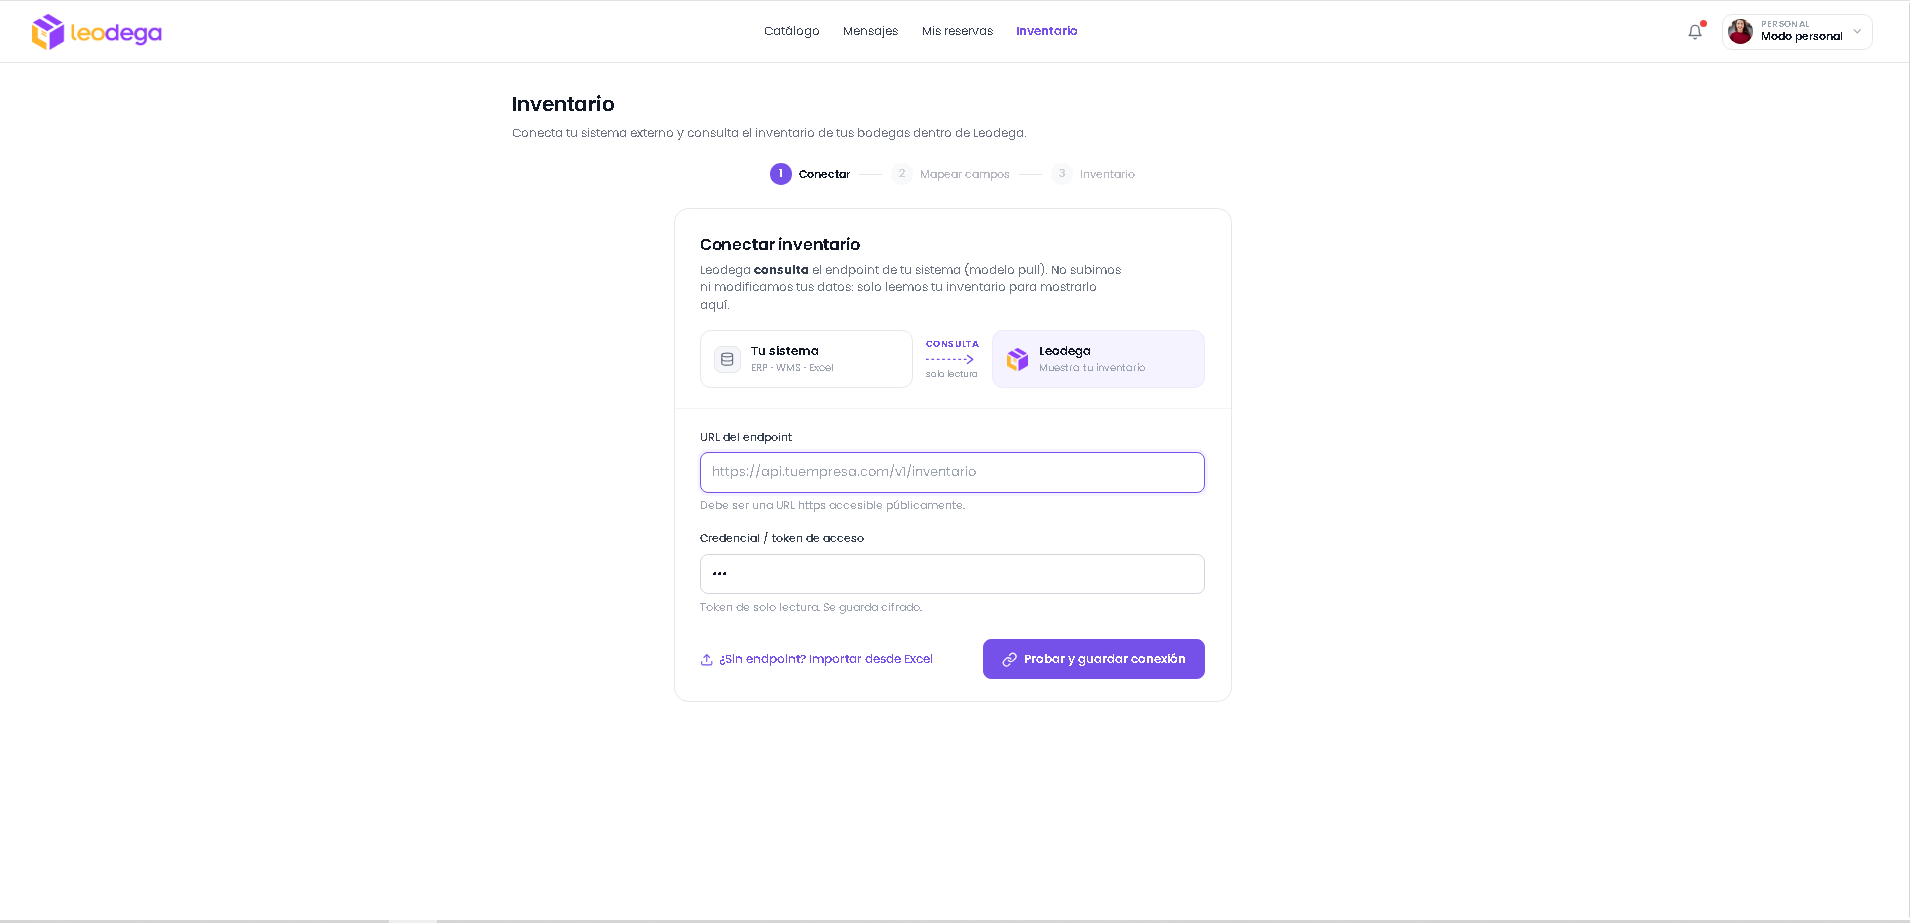
\includegraphics[width=\linewidth]{imagenes/fig14_inventory.png}
    \caption{Inventario: conexión a un sistema externo mediante URL de endpoint y token de acceso de solo lectura.}
    \label{fig:inventory}
\end{figure}
\clearpage

\subsubsection{Gestor de Almacenamiento (Arrendador)}
\noindent El rol de Gestor provee un panel de administración para publicar bodegas, dar seguimiento a las reservas entrantes, comunicarse con clientes y monitorear el calendario de ocupación.

\begin{figure}[H]
    \centering
    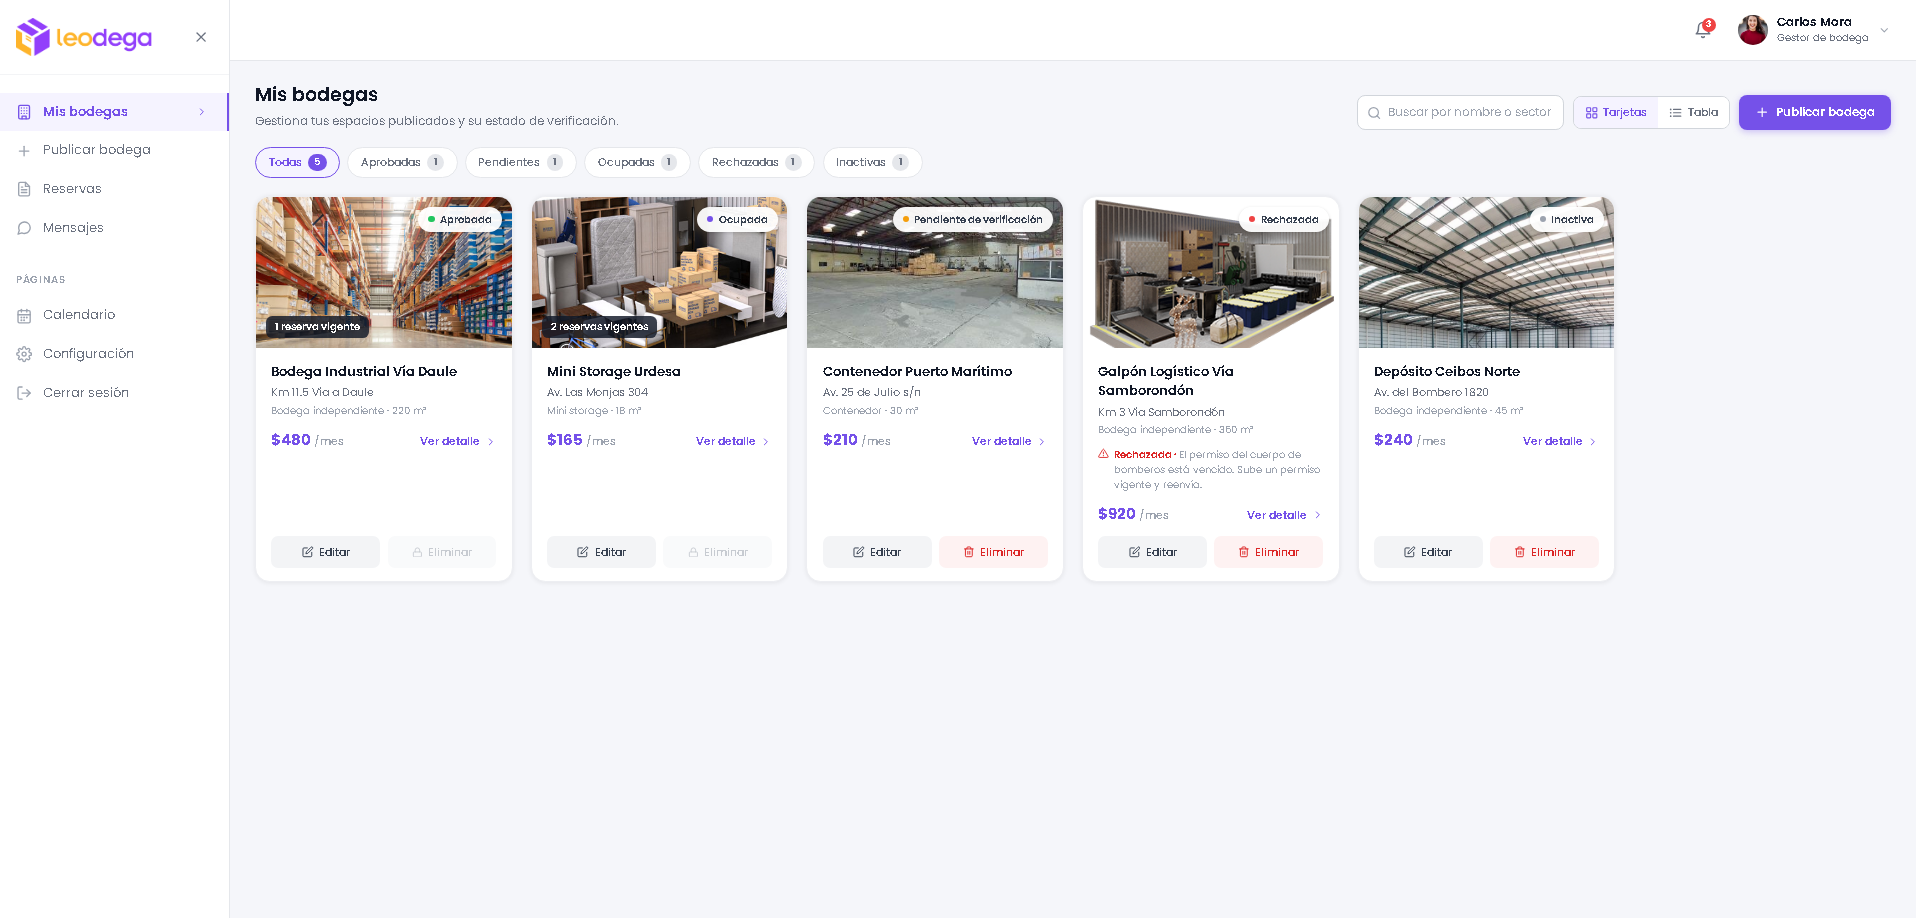
\includegraphics[width=\linewidth]{imagenes/fig15_my_warehouses_all.png}
    \caption{Mis Bodegas: panel principal con cinco bodegas en distintos estados de verificación.}
    \label{fig:my_warehouses_all}
\end{figure}

\begin{figure}[H]
    \centering
    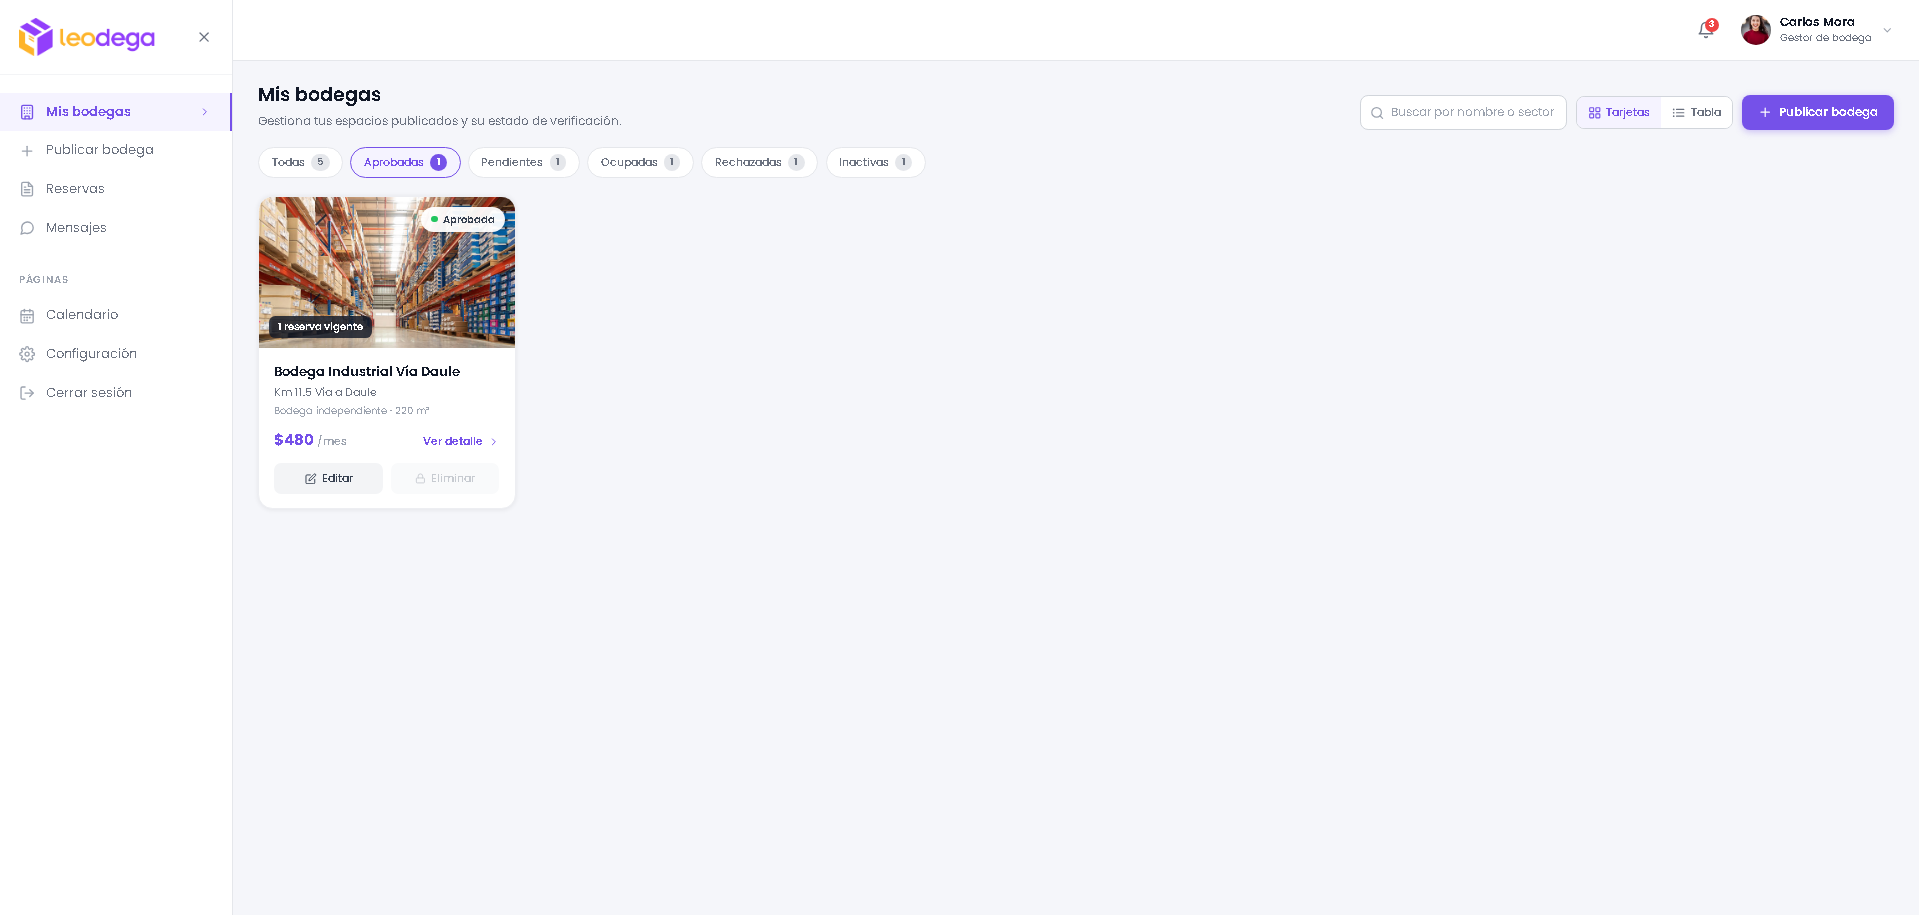
\includegraphics[width=\linewidth]{imagenes/fig16_my_warehouses_approved.png}
    \caption{Mis Bodegas: filtro ``Aprobadas'' mostrando una bodega activa con una reserva en curso.}
    \label{fig:my_warehouses_approved}
\end{figure}

\noindent\textbf{Publicar Bodega.} Flujo guiado de siete pasos para publicar una nueva bodega: tipo de espacio, modalidad de almacenamiento, fotos, ubicación, título y descripción, precio y tamaño, y documentación de seguridad.

\begin{figure}[H]
    \centering
    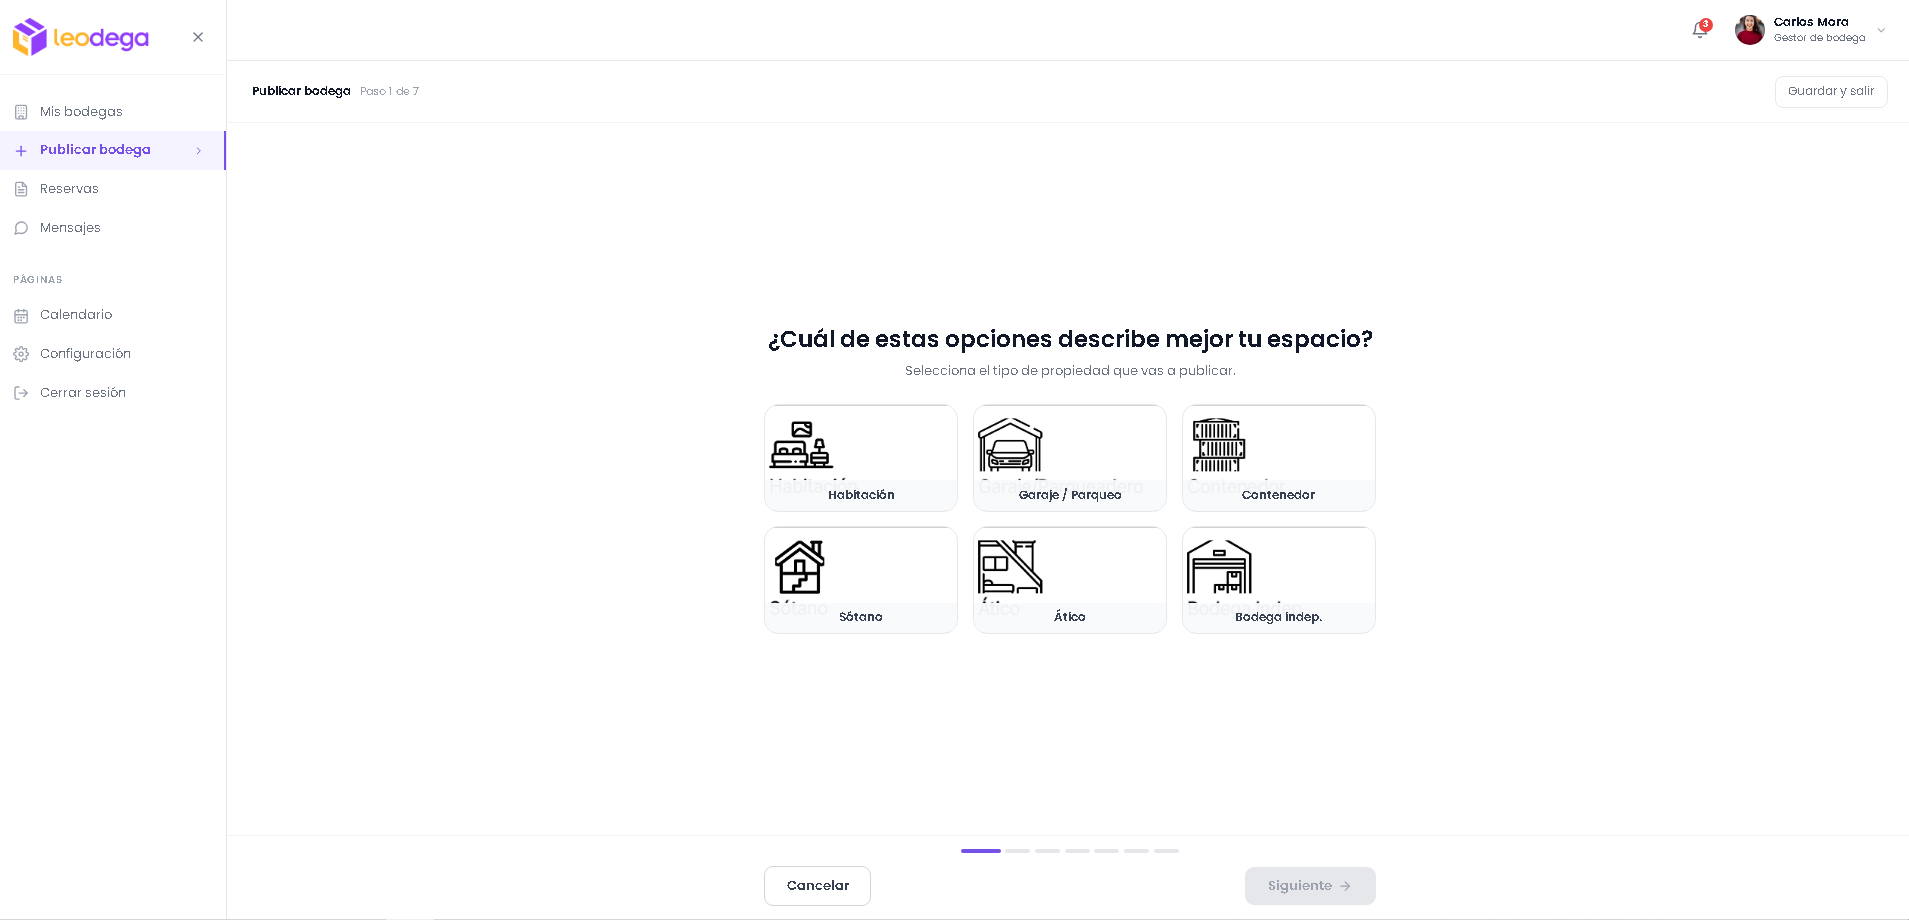
\includegraphics[width=\linewidth]{imagenes/fig17_publish_step1.png}
    \caption{Publicar Bodega, Paso 1/7: selección del tipo de espacio.}
    \label{fig:publish_step1}
\end{figure}

\begin{figure}[H]
    \centering
    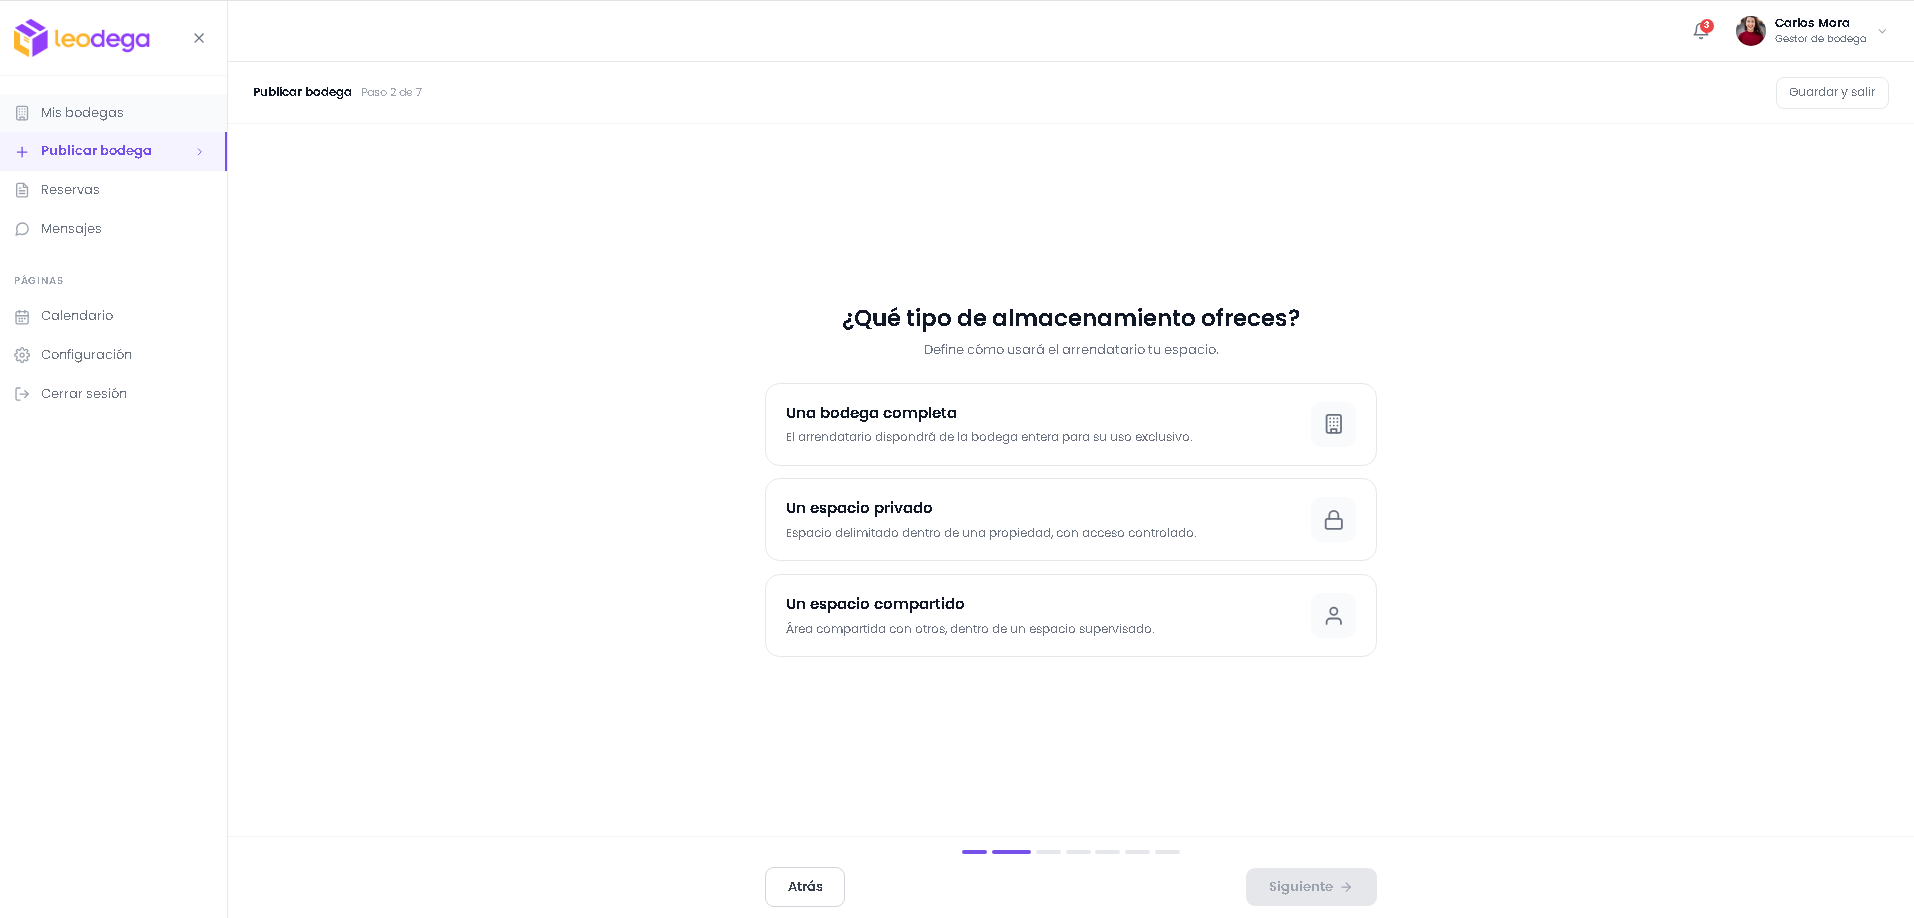
\includegraphics[width=\linewidth]{imagenes/fig18_publish_step2.png}
    \caption{Publicar Bodega, Paso 2/7: modalidad de almacenamiento (completo, privado o compartido).}
    \label{fig:publish_step2}
\end{figure}

\begin{figure}[H]
    \centering
    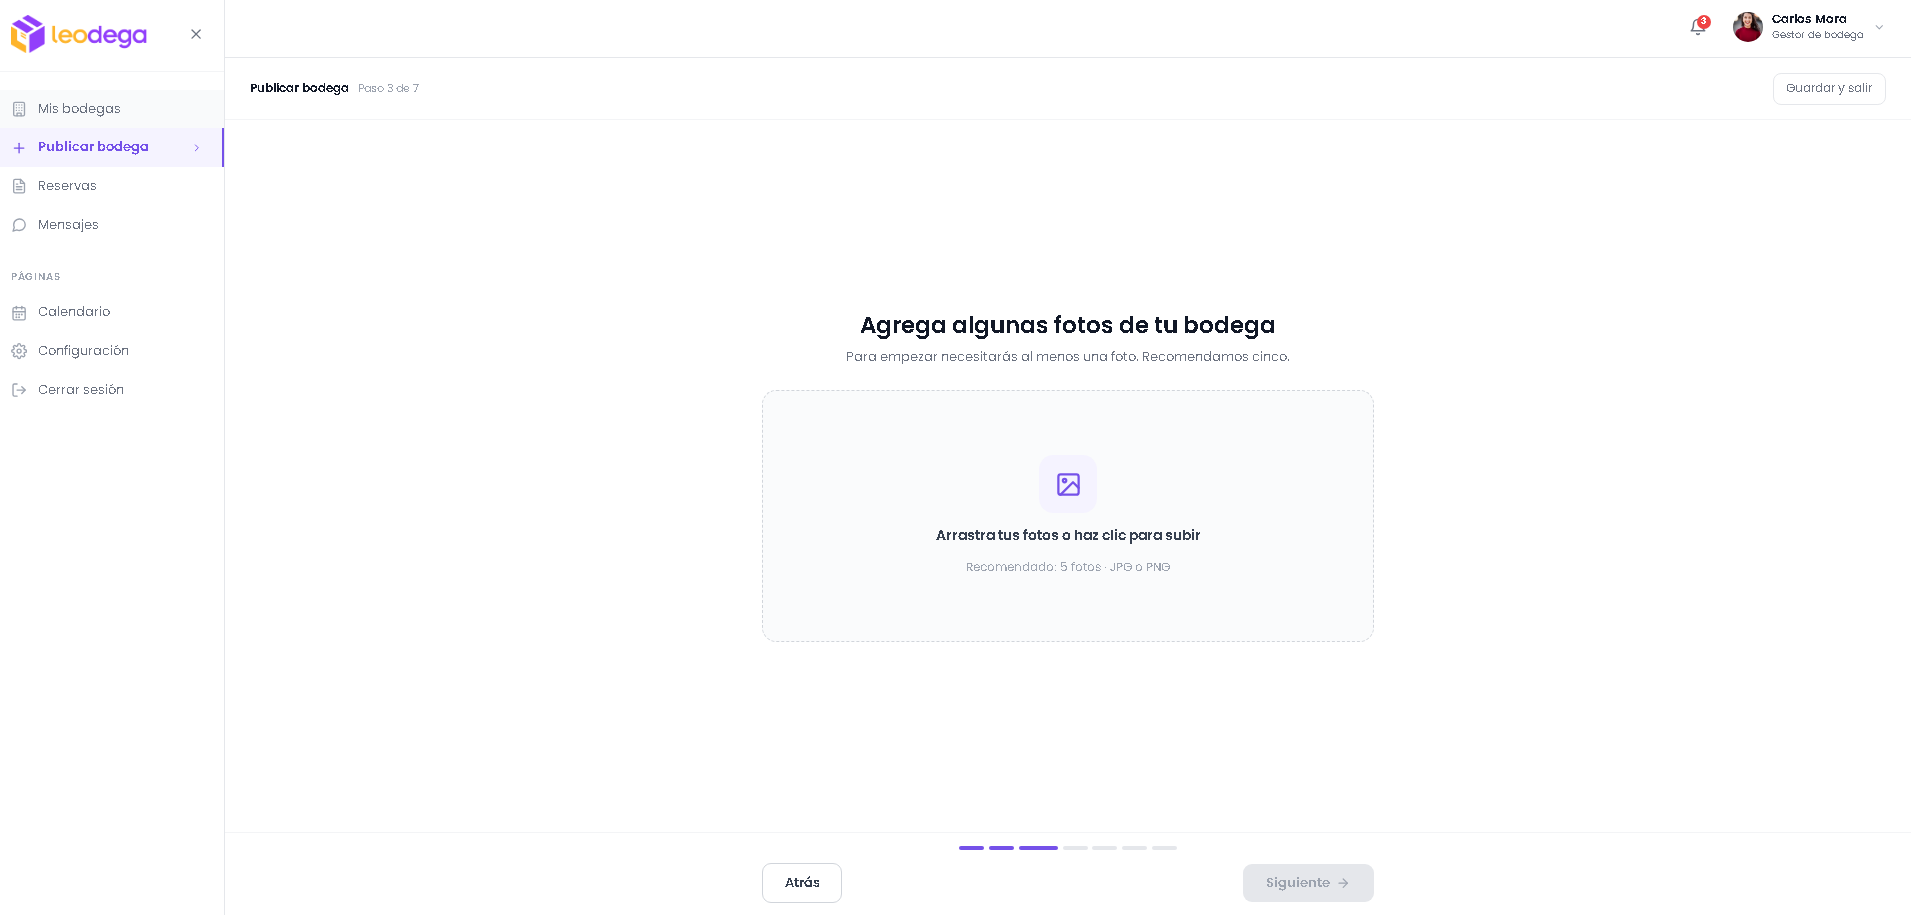
\includegraphics[width=\linewidth]{imagenes/fig19_publish_step3.png}
    \caption{Publicar Bodega, Paso 3/7: carga de fotos (mínimo 1, recomendado 5).}
    \label{fig:publish_step3}
\end{figure}

\begin{figure}[H]
    \centering
    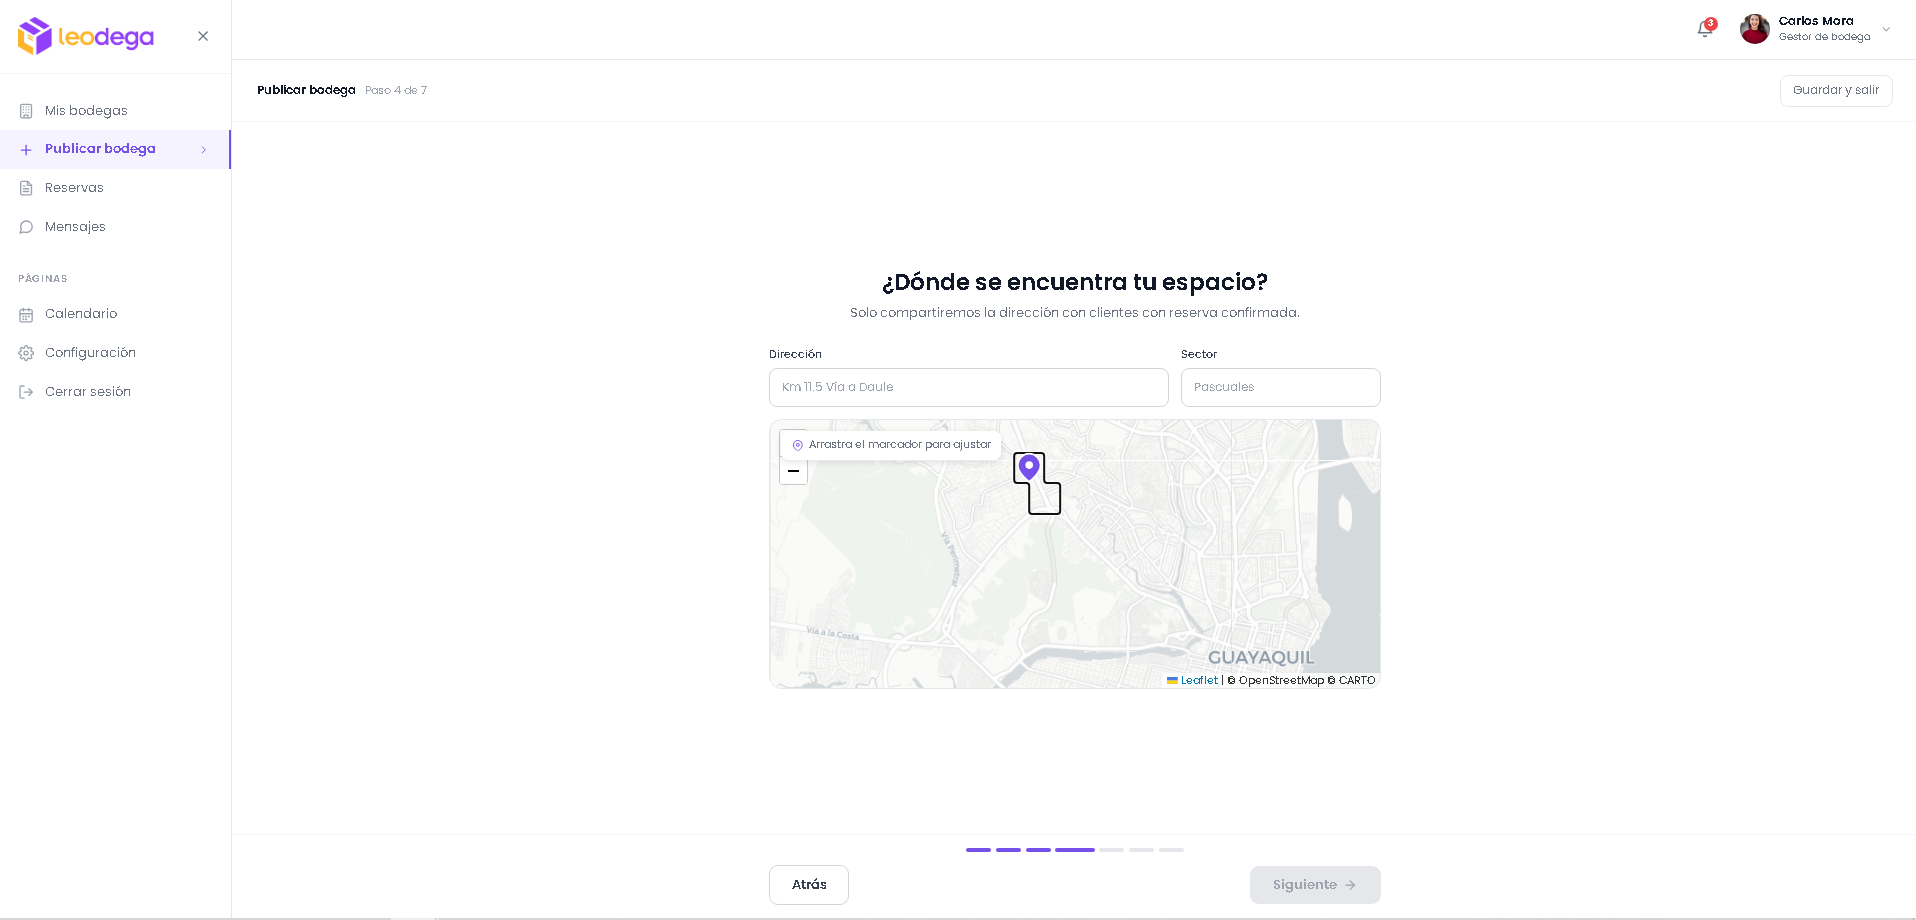
\includegraphics[width=\linewidth]{imagenes/fig20_publish_step4.png}
    \caption{Publicar Bodega, Paso 4/7: ubicación en el mapa con campos de dirección y distrito.}
    \label{fig:publish_step4}
\end{figure}

\begin{figure}[H]
    \centering
    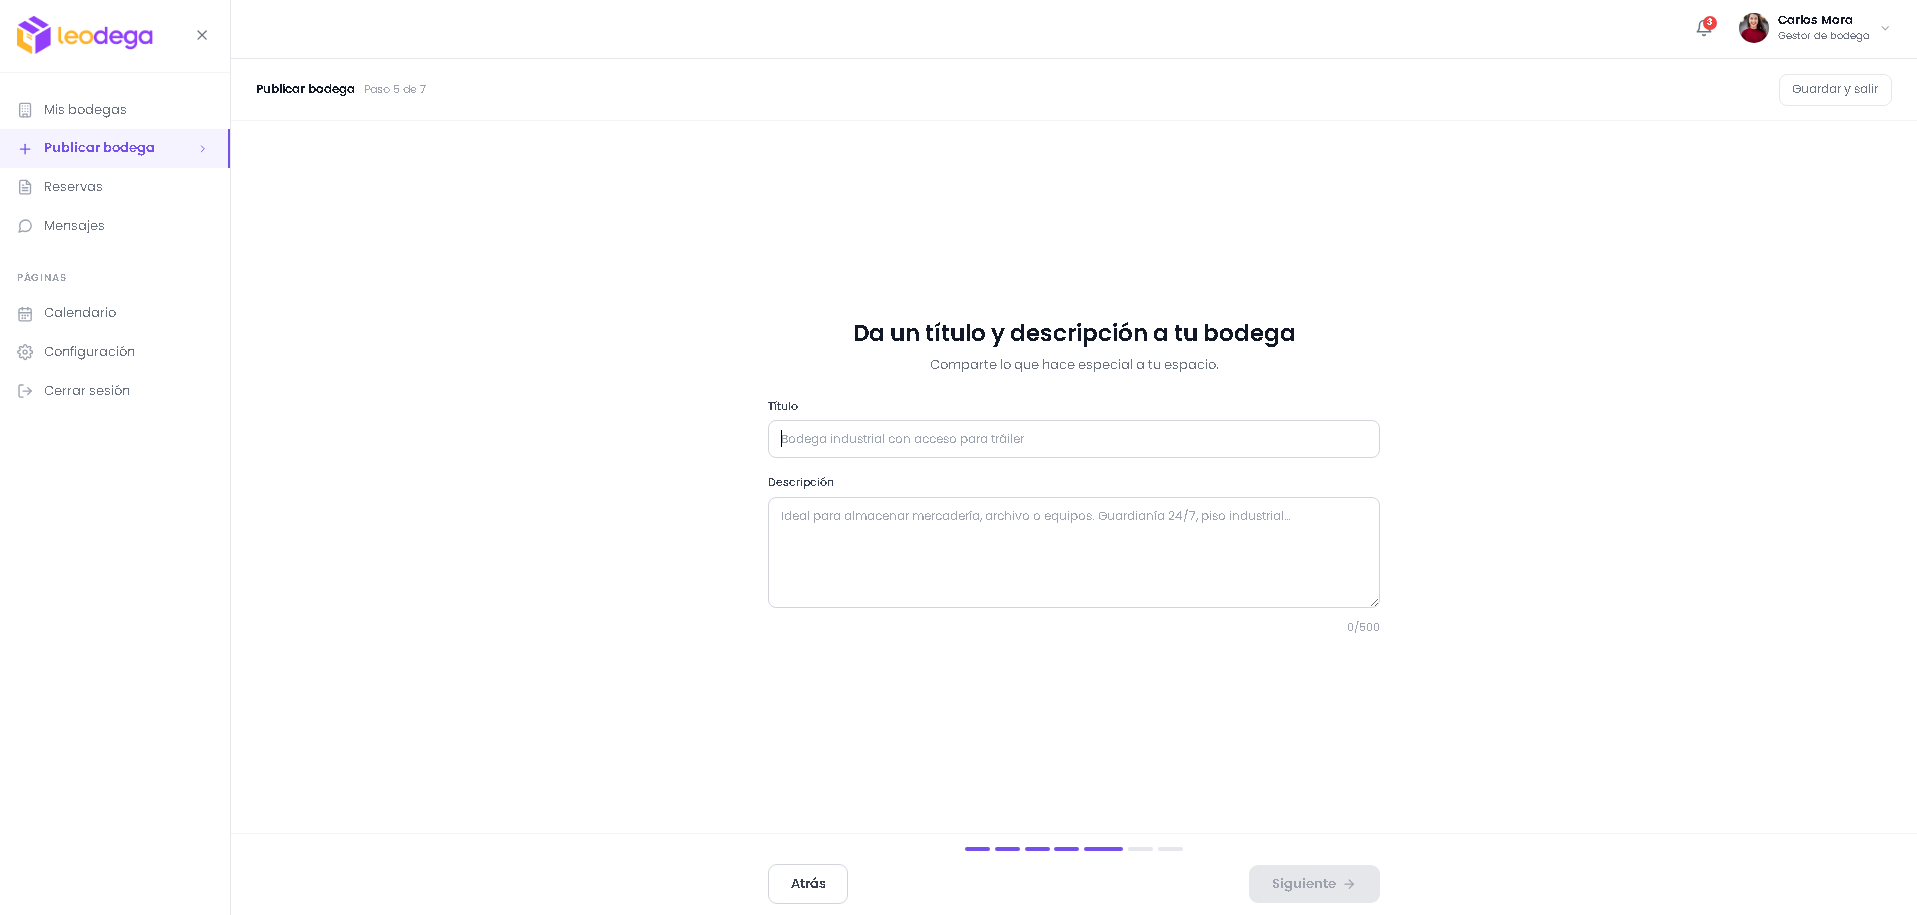
\includegraphics[width=\linewidth]{imagenes/fig21_publish_step5.png}
    \caption{Publicar Bodega, Paso 5/7: título y descripción del espacio.}
    \label{fig:publish_step5}
\end{figure}

\begin{figure}[H]
    \centering
    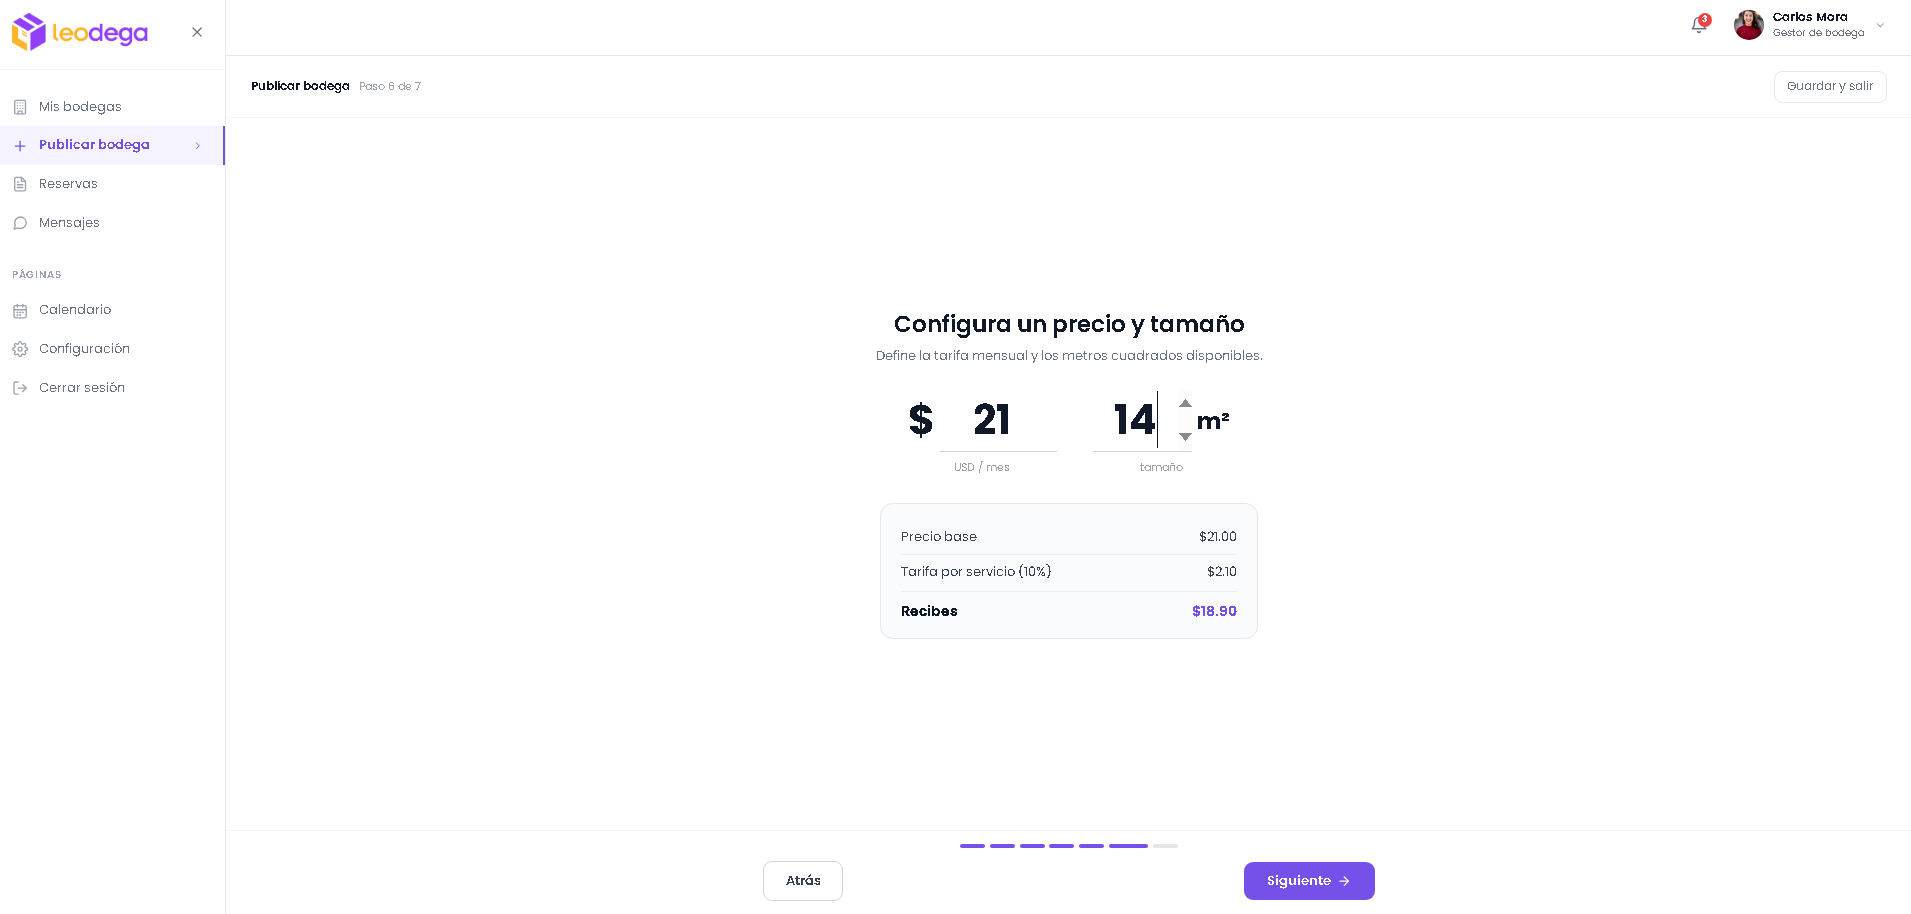
\includegraphics[width=\linewidth]{imagenes/fig22_publish_step6.png}
    \caption{Publicar Bodega, Paso 6/7: configuración de precio mensual y área en m$^{2}$.}
    \label{fig:publish_step6}
\end{figure}

\begin{figure}[H]
    \centering
    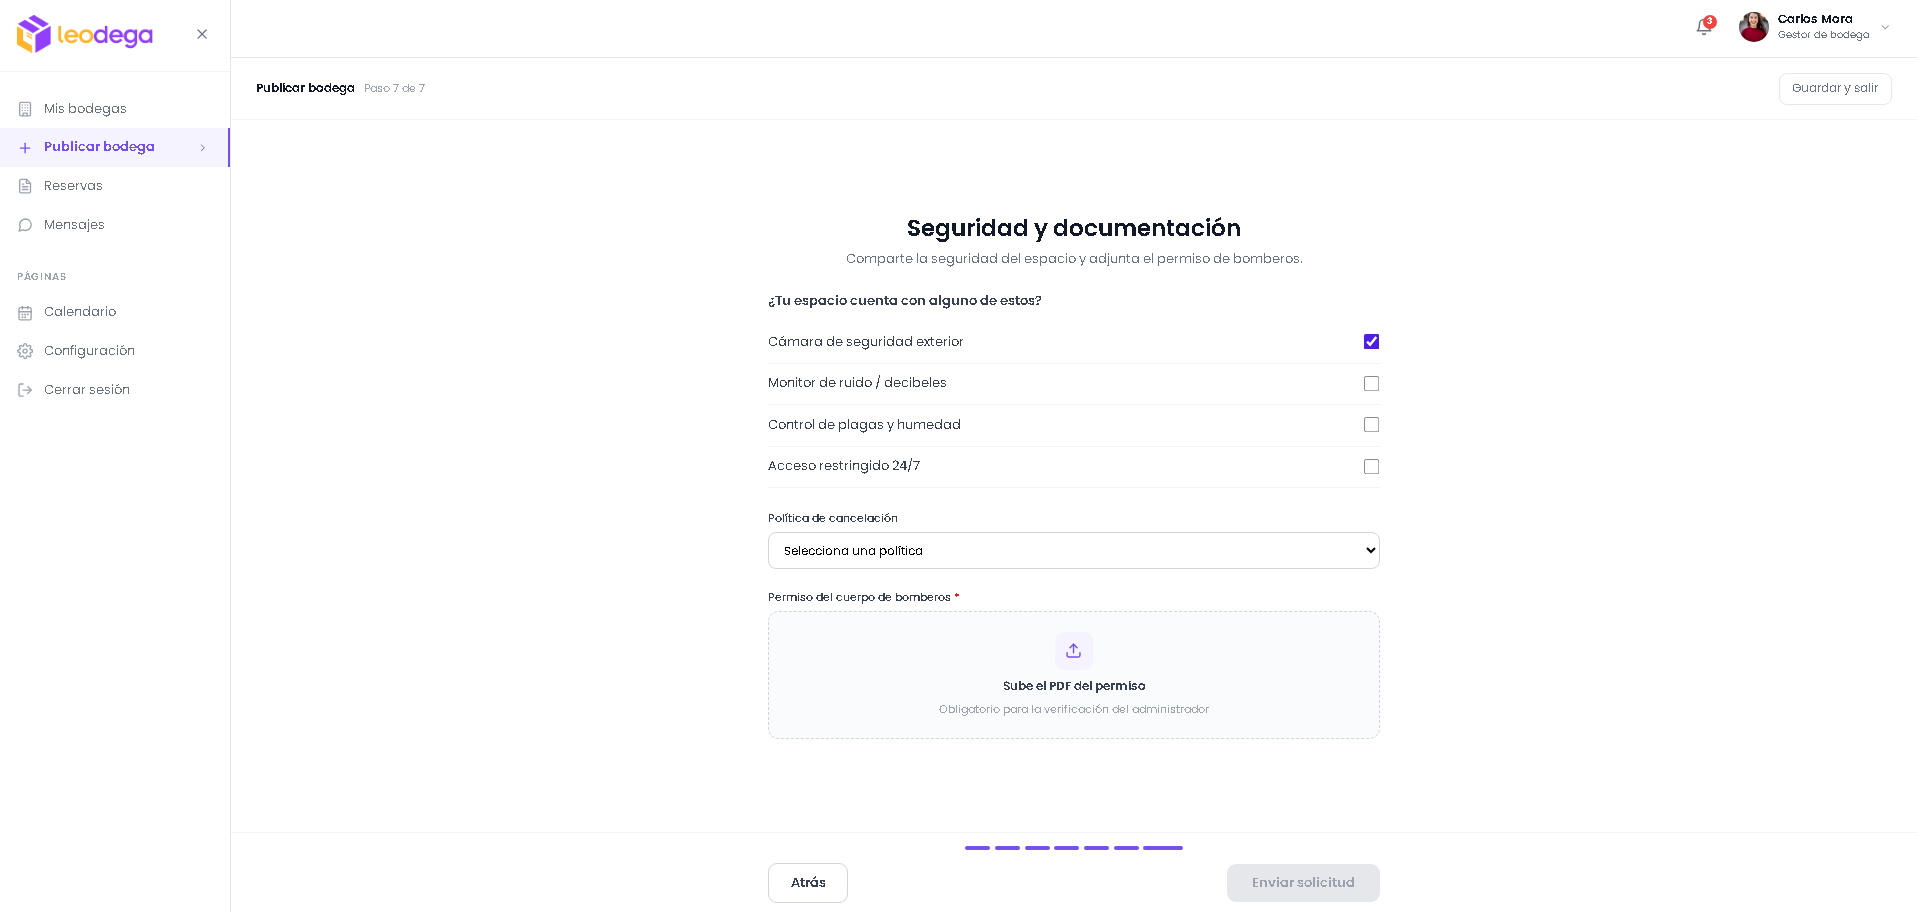
\includegraphics[width=\linewidth]{imagenes/fig23_publish_step7.png}
    \caption{Publicar Bodega, Paso 7/7: características de seguridad, política de cancelación y permiso de bomberos obligatorio.}
    \label{fig:publish_step7}
\end{figure}

\begin{figure}[H]
    \centering
    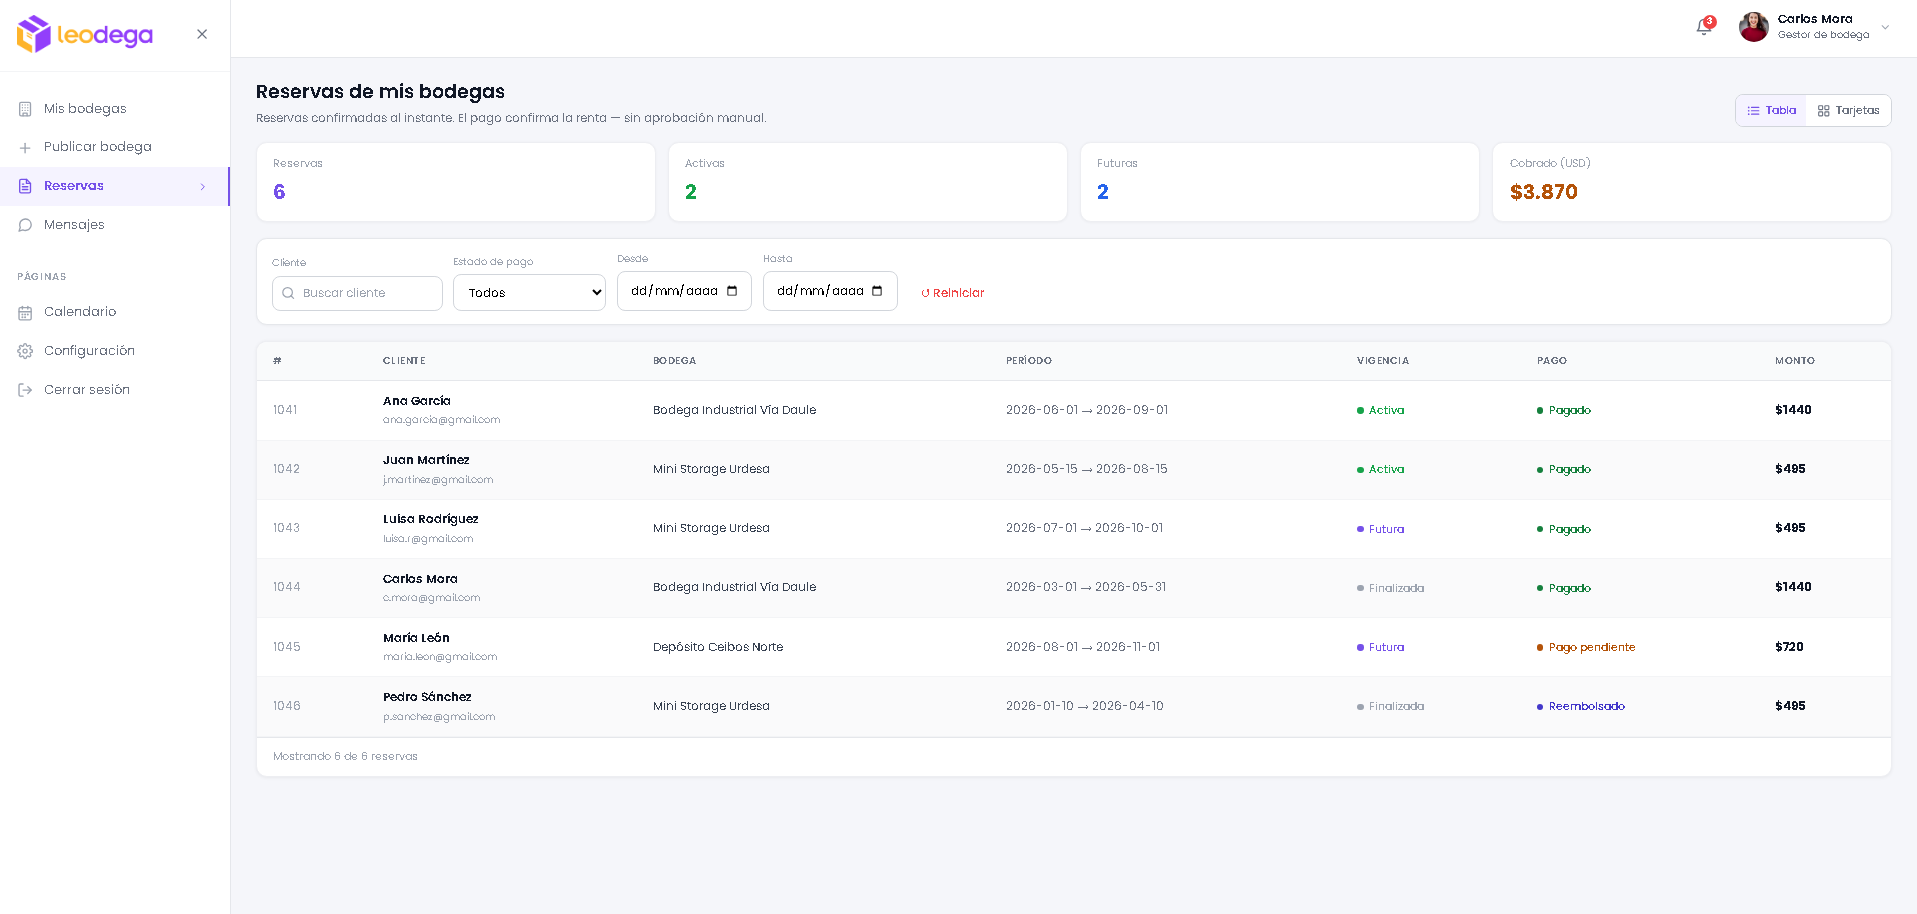
\includegraphics[width=\linewidth]{imagenes/fig24_manager_bookings.png}
    \caption{Reservas Recibidas: tabla con seis reservas, métricas globales y filtros por cliente, estado de pago y fecha.}
    \label{fig:manager_bookings}
\end{figure}

\begin{figure}[H]
    \centering
    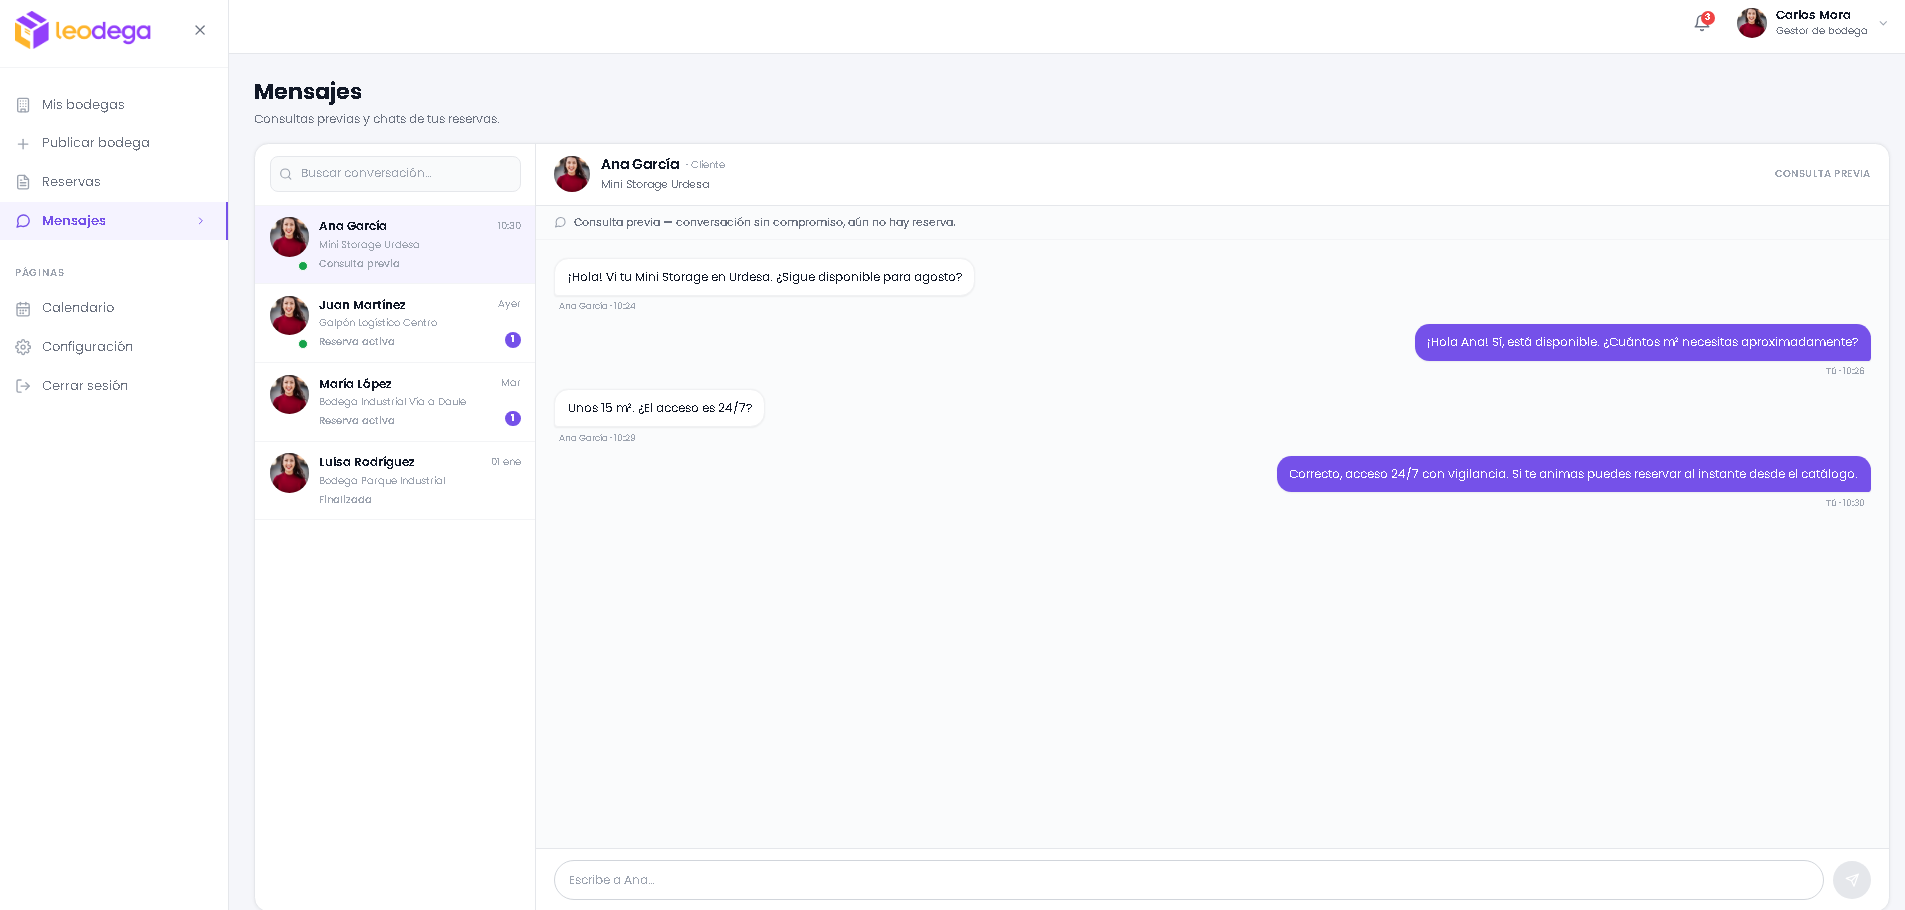
\includegraphics[width=\linewidth]{imagenes/fig25_manager_messages.png}
    \caption{Mensajes del Gestor: conversaciones con clientes organizadas por bodega y estado de la reserva.}
    \label{fig:manager_messages}
\end{figure}

\begin{figure}[H]
    \centering
    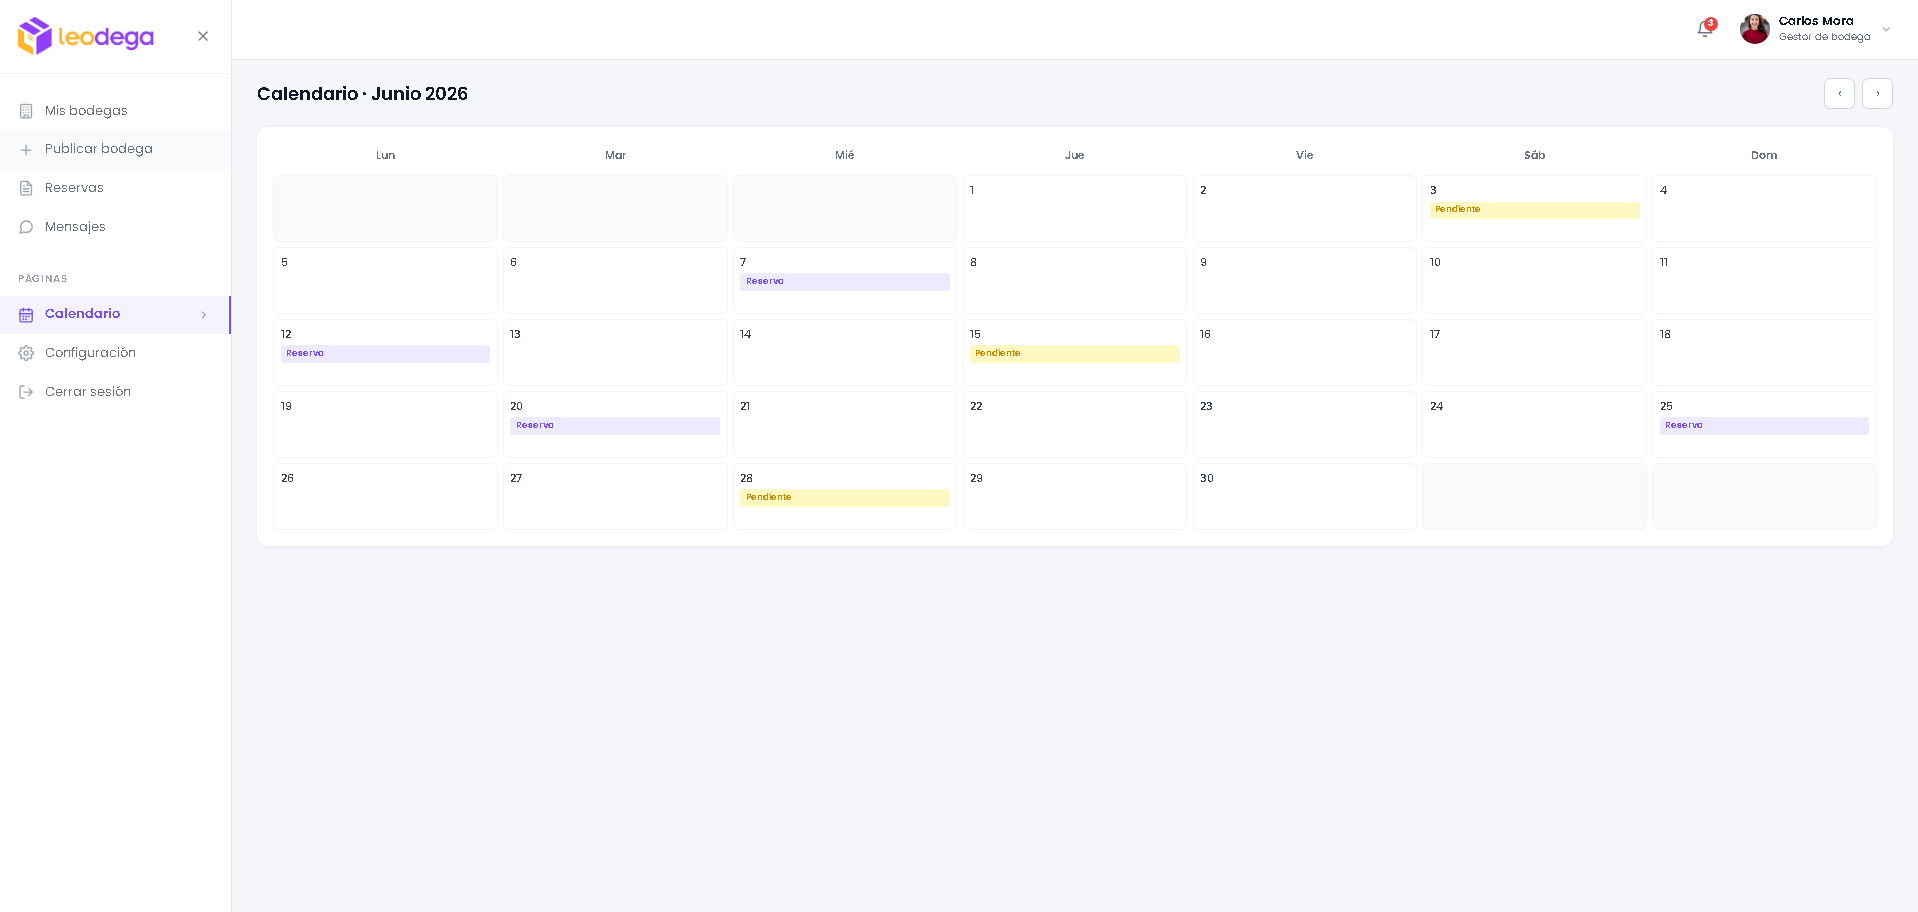
\includegraphics[width=\linewidth]{imagenes/fig26_calendar.png}
    \caption{Calendario: vista mensual (junio 2026) con reservas activas y eventos de pago pendiente.}
    \label{fig:calendar}
\end{figure}

\begin{figure}[H]
    \centering
    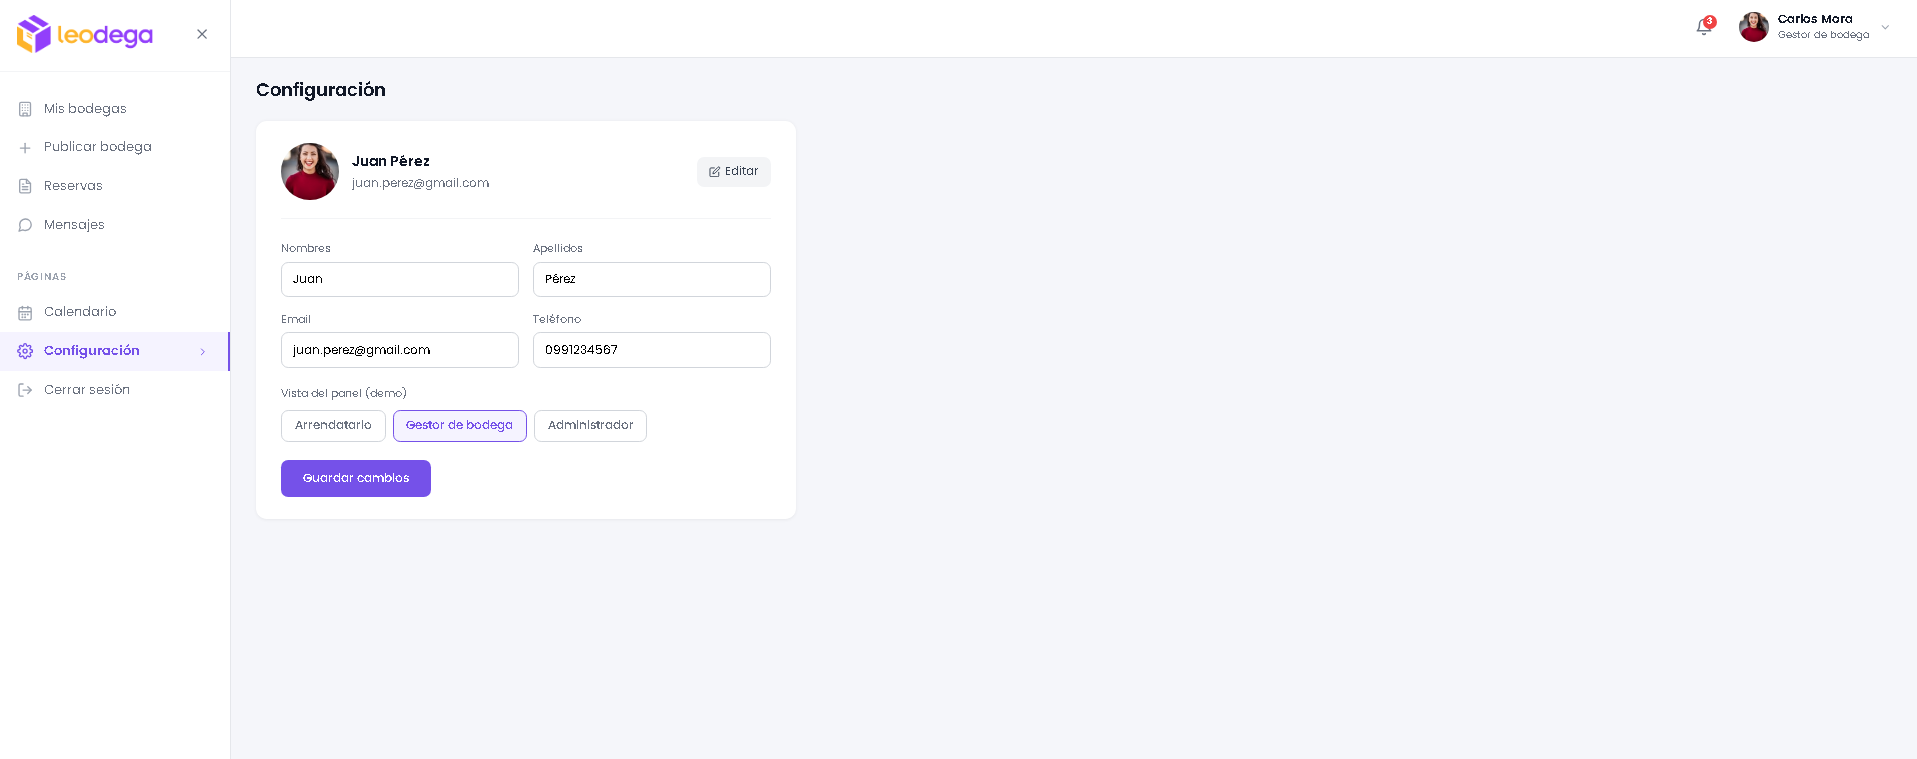
\includegraphics[width=0.55\linewidth]{imagenes/fig27_manager_config.png}
    \caption{Configuración de Perfil: editor de datos personales con selector de vista de rol.}
    \label{fig:manager_config}
\end{figure}
\clearpage

\subsubsection{Administrador}
\noindent El Administrador tiene control total de la plataforma: aprobación de publicaciones, gestión de cuentas de usuario, seguimiento de reportes de incidentes y mensajería directa con los participantes.

\begin{figure}[H]
    \centering
    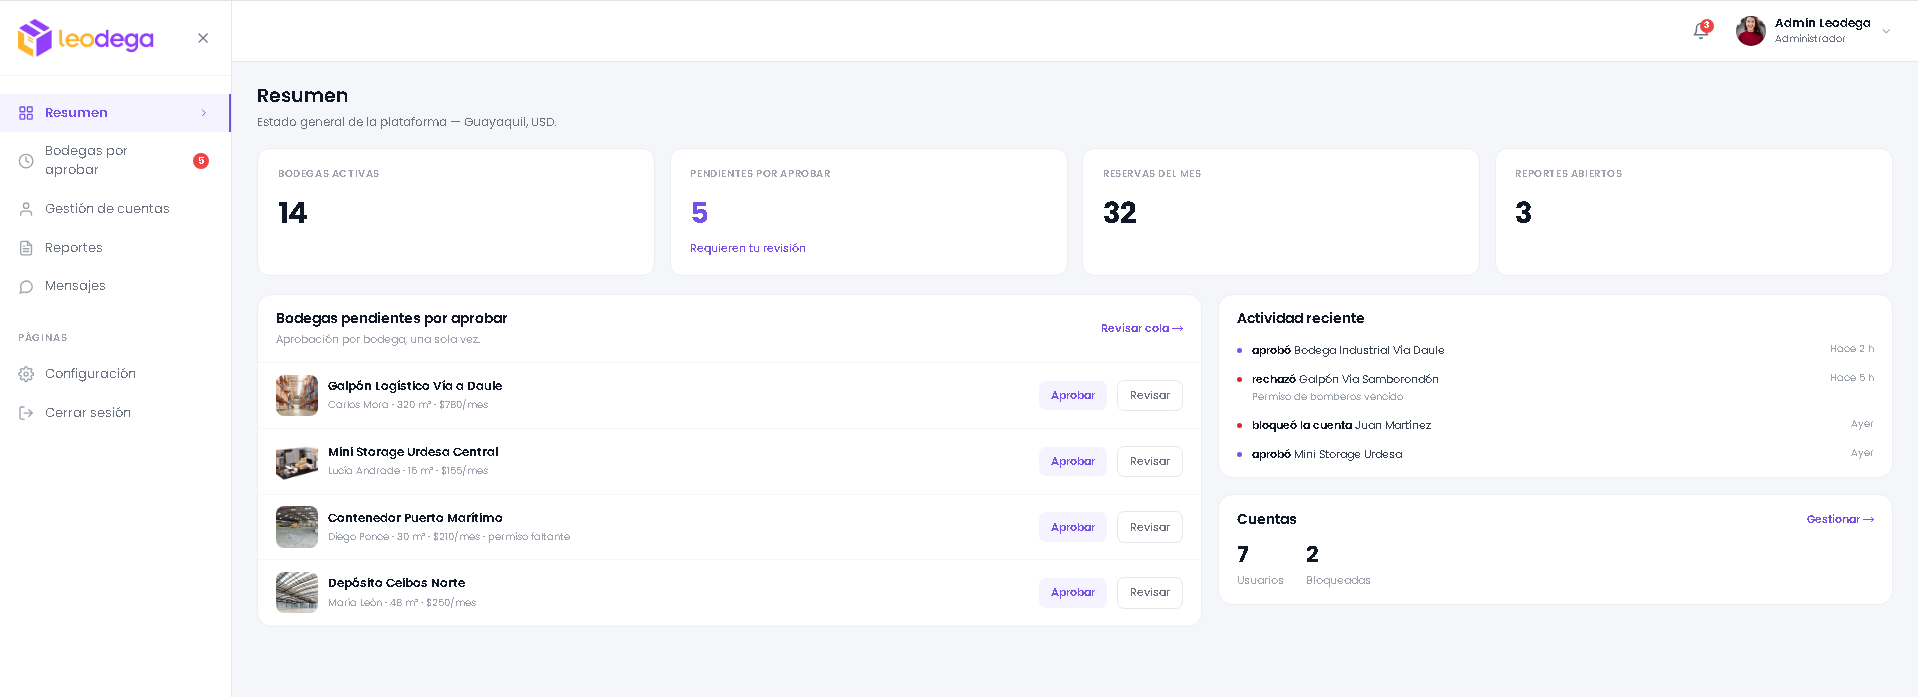
\includegraphics[width=\linewidth]{imagenes/fig28_admin_dashboard.png}
    \caption{Dashboard del Administrador: métricas globales -- 14 bodegas activas, 5 aprobaciones pendientes, 32 reservas y 3 reportes abiertos.}
    \label{fig:admin_dashboard}
\end{figure}

\begin{figure}[H]
    \centering
    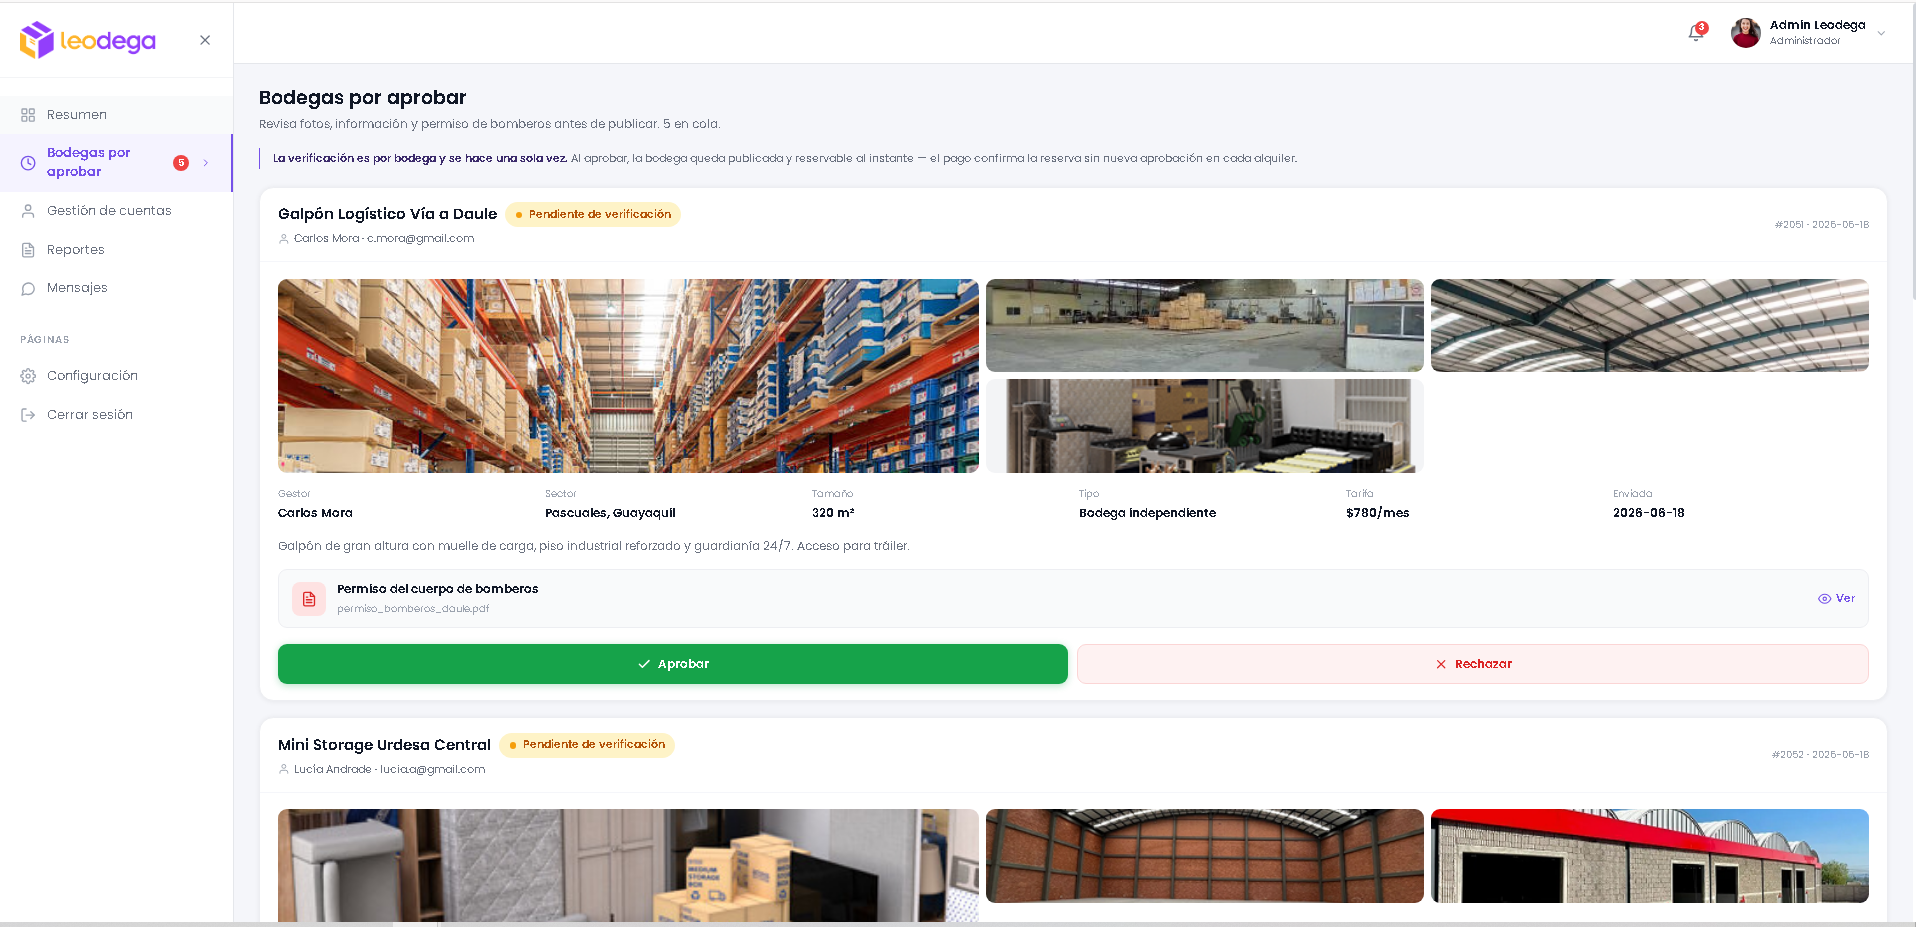
\includegraphics[width=\linewidth]{imagenes/fig29_admin_approval.png}
    \caption{Aprobación de Bodegas: cola de revisión con galería de fotos, detalles, verificación del permiso y acciones de aprobar/rechazar.}
    \label{fig:admin_approval}
\end{figure}

\begin{figure}[H]
    \centering
    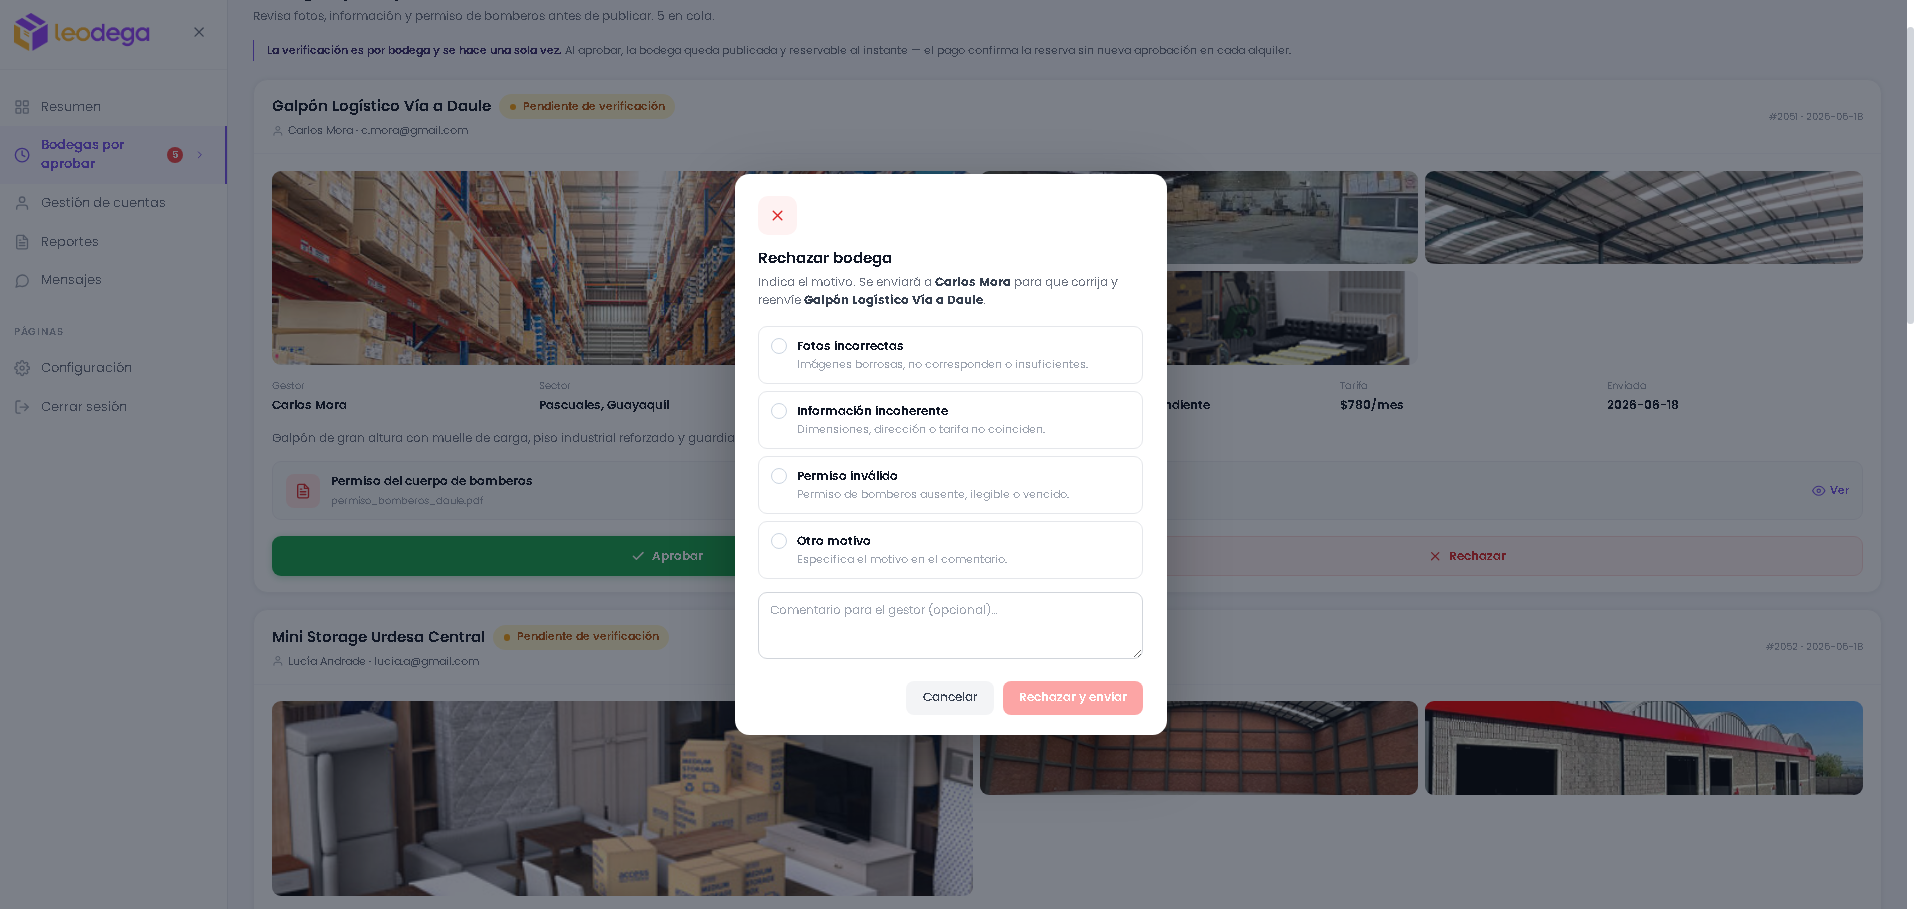
\includegraphics[width=\linewidth]{imagenes/fig30_admin_reject_modal.png}
    \caption{Modal de Rechazo de Bodega: selección de la razón de rechazo con comentario opcional enviado al gestor.}
    \label{fig:admin_reject_modal}
\end{figure}

\begin{figure}[H]
    \centering
    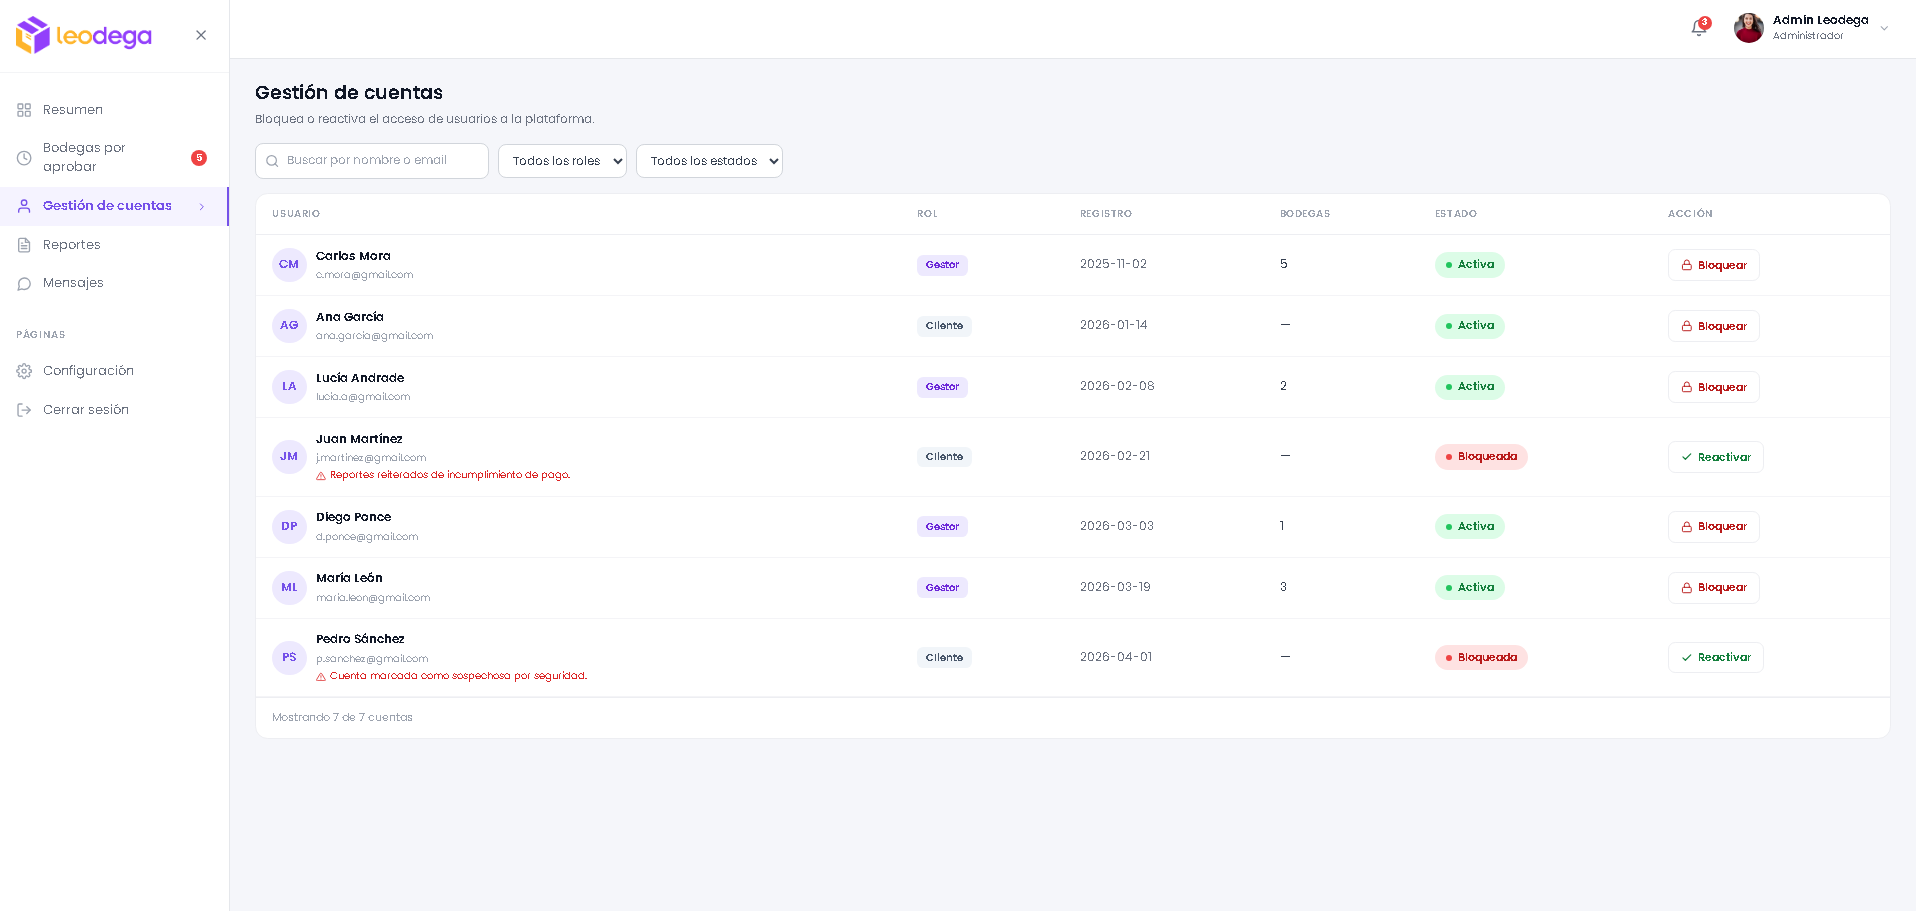
\includegraphics[width=\linewidth]{imagenes/fig31_admin_accounts.png}
    \caption{Gestión de Cuentas: tabla de usuarios con rol, fecha de registro, número de bodegas y estado de la cuenta.}
    \label{fig:admin_accounts}
\end{figure}

\begin{figure}[H]
    \centering
    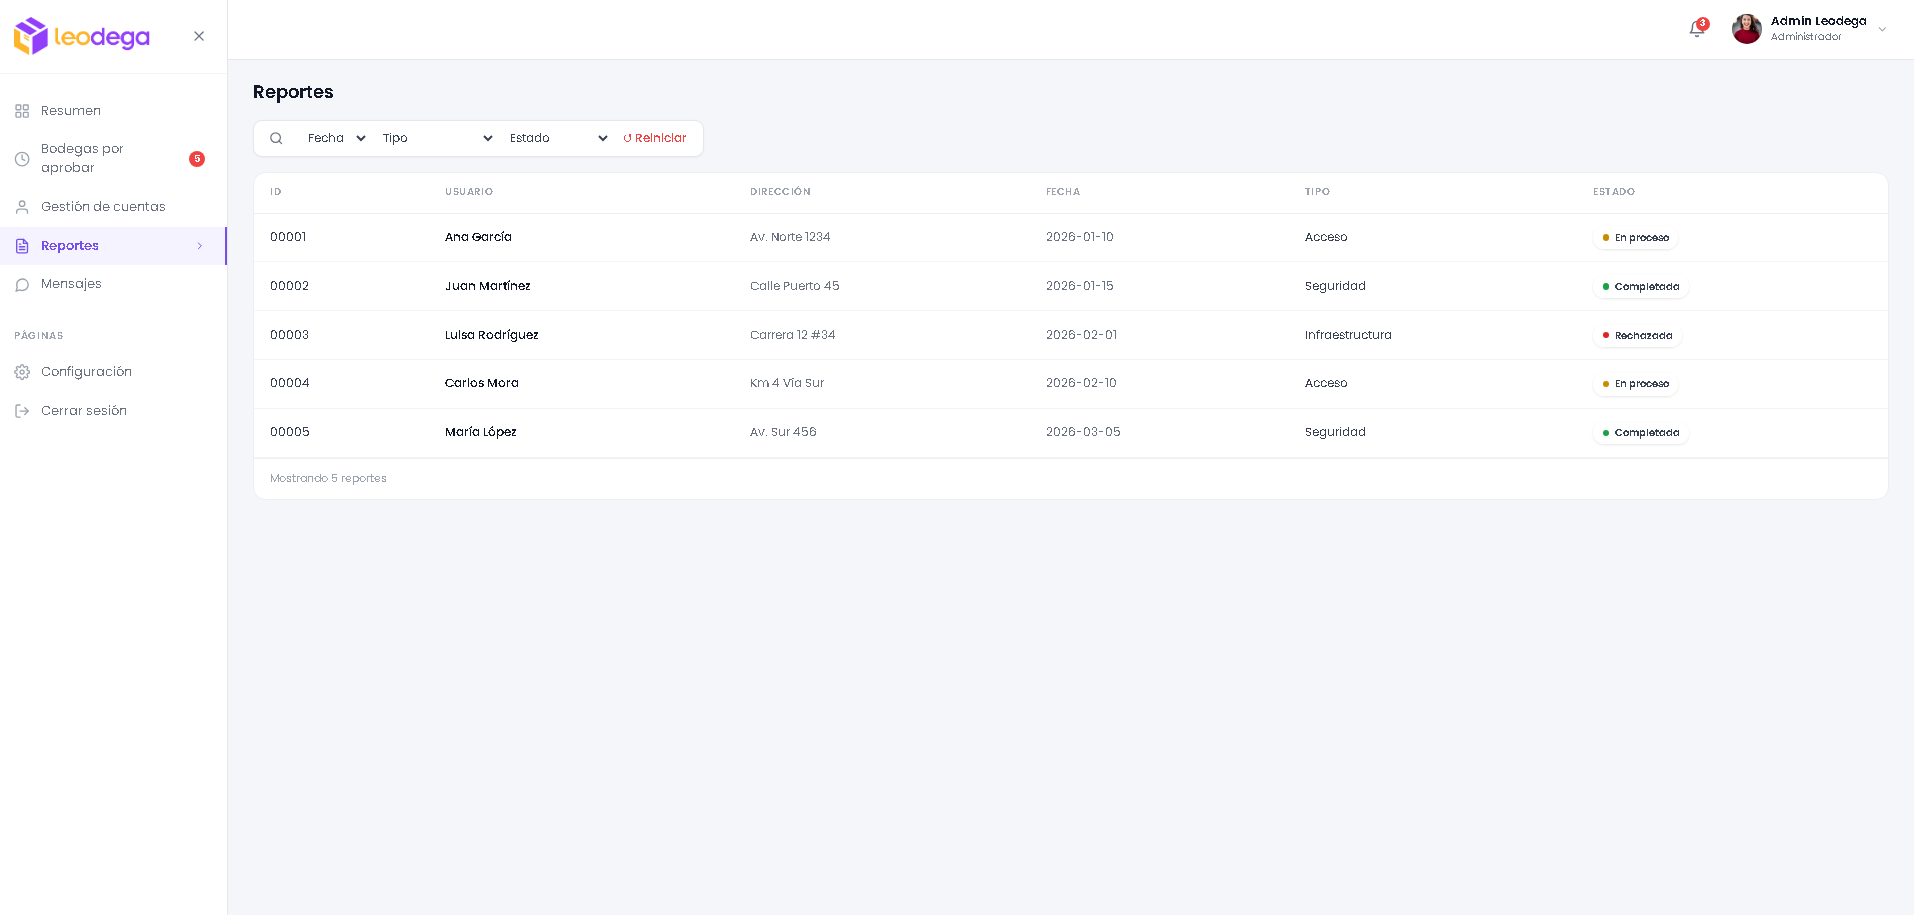
\includegraphics[width=\linewidth]{imagenes/fig32_admin_reports.png}
    \caption{Reportes: tabla de incidentes con usuario, dirección, fecha, tipo y estado de resolución.}
    \label{fig:admin_reports}
\end{figure}

\begin{figure}[H]
    \centering
    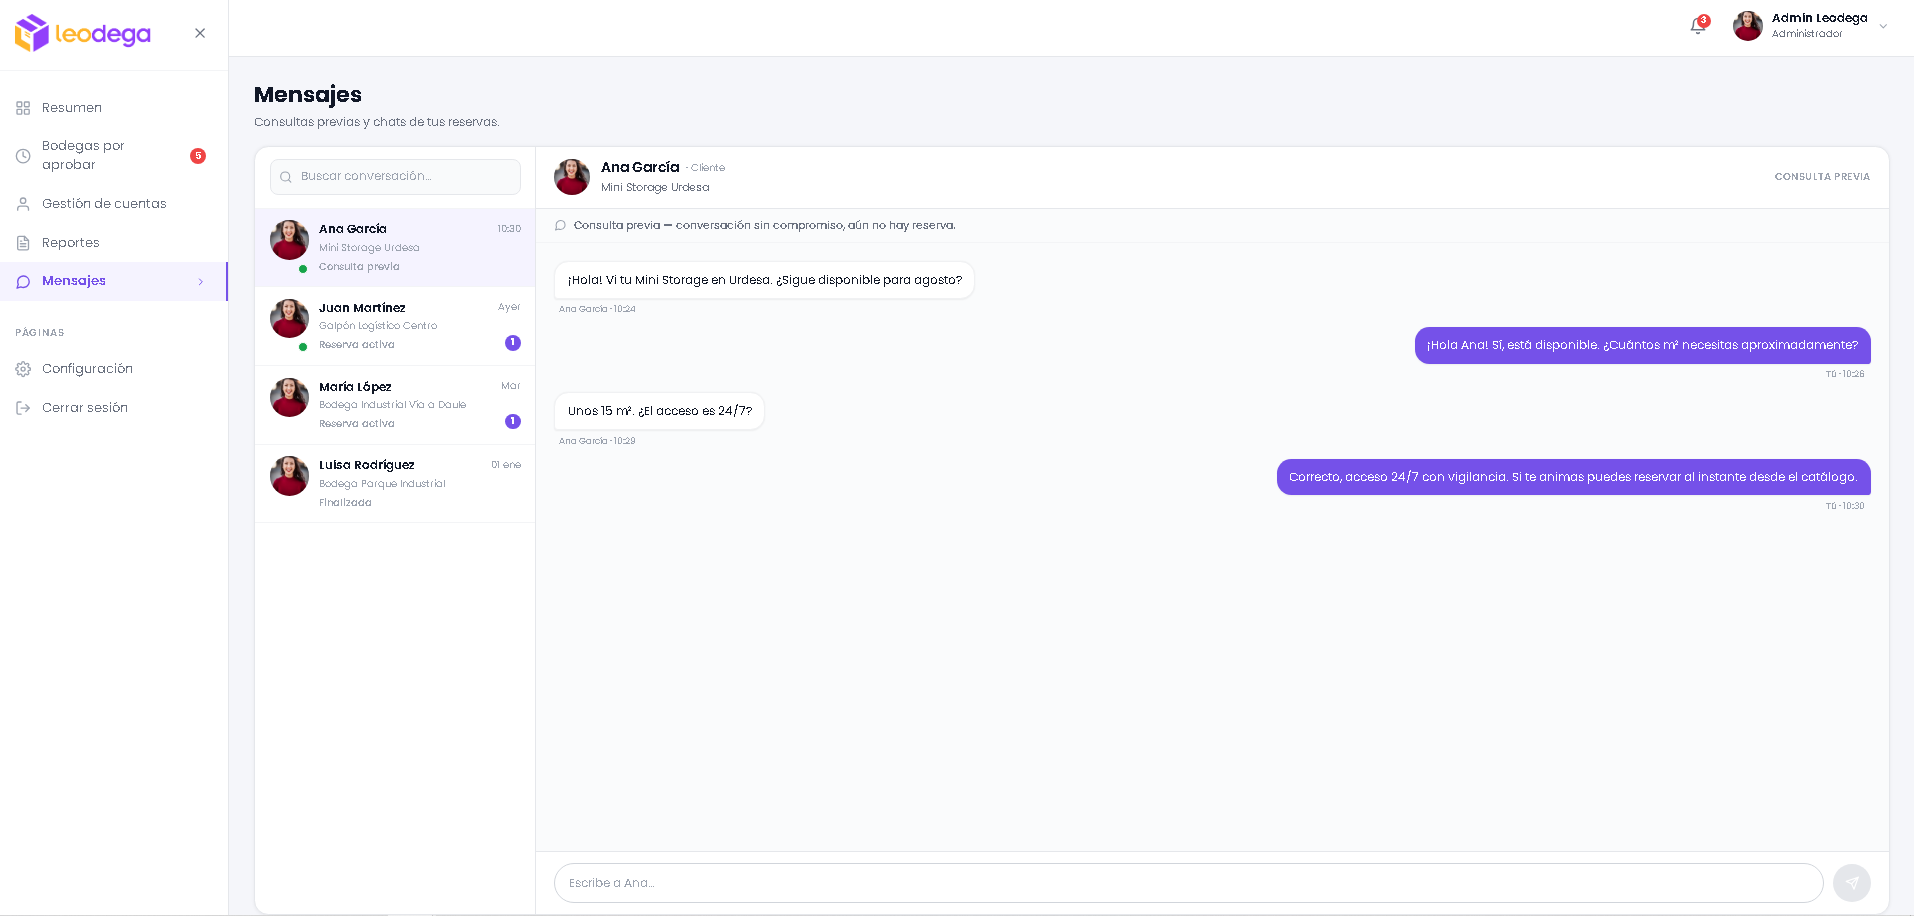
\includegraphics[width=\linewidth]{imagenes/fig33_admin_messages.png}
    \caption{Mensajes del Administrador: bandeja de conversaciones con usuarios para soporte y moderación.}
    \label{fig:admin_messages}
\end{figure}

\begin{figure}[H]
    \centering
    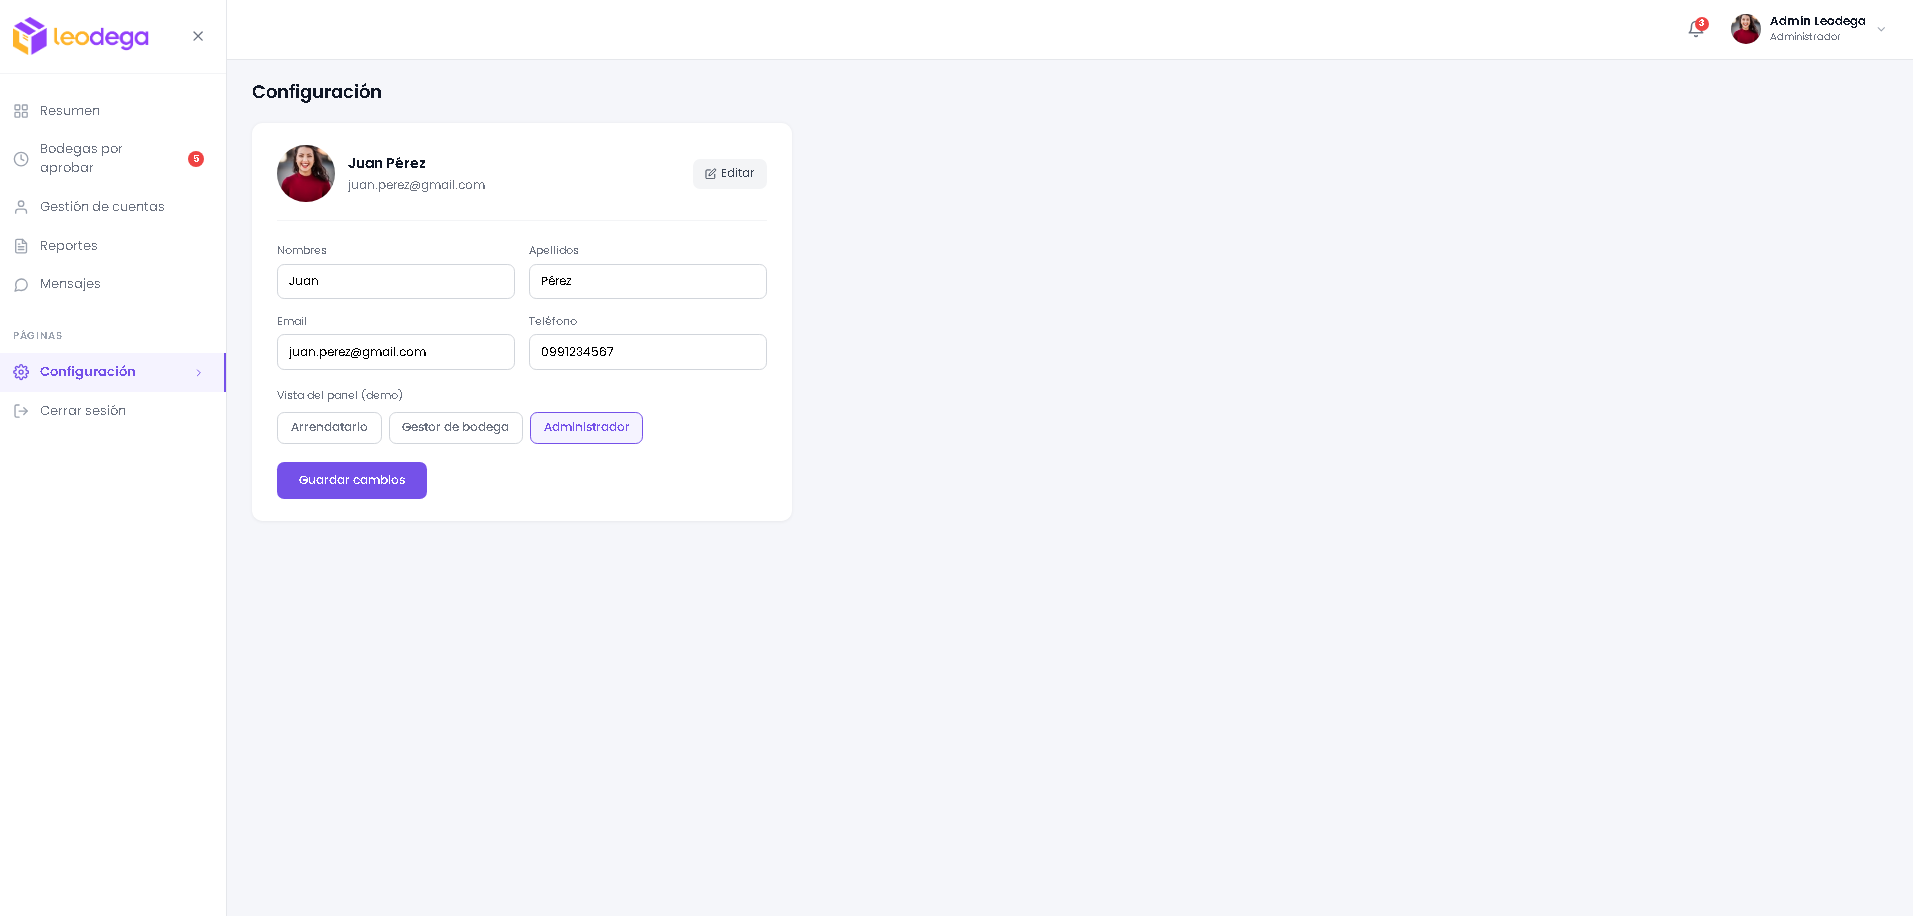
\includegraphics[width=0.55\linewidth]{imagenes/fig34_admin_config.png}
    \caption{Configuración de Perfil del Administrador: editor de datos personales con selector de vista de rol.}
    \label{fig:admin_config}
\end{figure}
\clearpage
